\documentclass[journal,sort]{IEEEtran}

\usepackage{lineno,hyperref}
\usepackage{bm}
\usepackage{cancel}
\usepackage{booktabs}
\usepackage{multirow}
\usepackage{array,chngpage}
\usepackage{subfigure}
\usepackage{amssymb}
\usepackage{graphicx}
\usepackage{amsmath}
\usepackage{bm}
\usepackage{diagbox}
\usepackage{cite}
\usepackage{threeparttable}
\usepackage{url}
\usepackage{setspace}
\usepackage{caption}
\DeclareMathOperator*{\argmax}{argmax}
\usepackage[linewidth=1pt]{mdframed}
\usepackage{lipsum}
\usepackage{booktabs}
\usepackage{color}
\usepackage{longtable}


\bibliographystyle{IEEEtran}

\begin{document}


% first the title is needed
\title{Detection of Double Compression with the Same Coding Parameters Based on Quality Degradation Mechanism Analysis \thanks{This work is supported by the National Natural Science Foundation of China (No. 61572320, 61572321). P. He received financial support from China Scholarship Council (CSC) for the Scholarship Fund No.[2016]3100 program.}
\thanks{X. Jiang, P. He, T. Sun, F. Xie and S. Wang are with the School of Electronic Information and Electrical Engineering, Shanghai Jiao Tong University, Shanghai, China (e-mail: \{xhjiang, gokeyhps, tfsun, 190432944, wsl\}@sjtu.edu.cn). The corresponding author is Dr. Tanfeng Sun.}}	


\author{Xinghao~Jiang,~\IEEEmembership{Member,~IEEE,}
	Peisong~He,~\IEEEmembership{Student Member,~IEEE,}
	Tanfeng~Sun,~\IEEEmembership{Member,~IEEE,}%~\IEEEmembership{Fellow,~OSA,}
	~Feng~Xie,
	and~Shilin~Wang}

\maketitle



\begin{abstract}
Detection of double compression with the same coding parameters is a very challenging problem in video forensics, since traces of recompression operations are extremely slight in this case. To solve this problem, we first analyze degradation mechanisms during recompression. It is observed that video quality tends to become nearly unchanged after multiple recompressions with the same coding parameters. The degree of quality degradation is used to distinguish single and double compressed videos. This property can be described using the convergent tendency of video data to unchanged states after continuous recompressions. For MPEG videos, statistical features of rounding and truncation errors are extracted from the intra-coding process while macroblock-mode based features are obtained from the inter-coding process. The final feature is generated by concatenating these two sets of features to provide robust detection capability. Then, extracted features are fed to the SVM classifier to obtain the final detection result. Additionally, aforementioned features are modified and extended to detect double compression on H.264 videos based on the unique coding techniques developed in the H.264 standard, such as intra-prediction. Several public available YUV sequences are used to construct double compression databases with three popular coding standards, including MPEG-2, MPEG-4 and H.264. In experiments, the proposed method outperforms several state-of-the-art methods for different compression qualities and rate control schemes. Experimental results demonstrate the proposed method has more robust detection capability of double compression under various encoding configurations. 
 

\end{abstract}

\begin{IEEEkeywords}
		double video compression, the same coding parameters, quality degradation, macroblock mode
\end{IEEEkeywords}


\section{Introduction\label{intro}}

Double compression on videos denotes a digital video (in the lossy compression format) has been compressed once again by the same or different lossy compression process. Similar to double JPEG compression in image forensics \cite{barni2016adversary,li2015revealing,li2015statistical}, detection of double compression on videos is a significant research issue in multimedia forensics. The trace of double compression is useful to recover compression history and locate tampering points of a query video \cite{chen2016automatic,aghamaleki2016inter}. The authentication analysis of suspicious videos is important especially in the court of law. Different from double JPEG compression, the properties of double compression on videos are more complicated due to the rich and varied options of video coding parameters. In most cases, people may introduce a new GOP structure or another video codec in the recompression process using default settings of video editing software. In recent years, some successful approaches have been proposed for detecting double compression on videos when the primary compression and the secondary compression have different coding parameter settings. For double compression with different compression qualities (namely, quality scales in variant bit rate (VBR) videos or the average bitrates in constant bit rate (CBR) videos), most of the researchers address this issue by exposing abnormal statistics of quantized DCT coefficients in both intra-coded frames (e.g. I-frames) and inter-coded frames (e.g. P-frames) \cite{chen2009detection,wang2009exposing,su2010detection,liao2011double,sun2012exposing,jiang2013detection}. For double compression with shifted GOP structures, researchers pointed out that periodical spikes of the relocated I-frame can be observed under several measurements \cite{vazquez2012detection,stamm2012temporal,he2015double,he2016double,he2017detection,he2017frame}, where relocated I-frame denotes original I-frame which is re-encoded as a P-frame in the secondary compression. Finally, for double compression with altered codecs, P. Bestagini et. al proposed a detection framework based on the idempotent property of lossy coding \cite{bestagini2012video,bestagini2013video,bestagini2016codec}. Their methods achieved a promising performance of detecting double compression with altered codecs. 

Unfortunately, for sophisticated forgers, it is easy to access the coding information in original video streams, such as the type of codec and compression quality. To avoid leaving obvious traces of the recompression operation, they are more likely to re-encode the tampered video with the same coding parameters as the original video. Therefore, existing methods designed for double compression with different compression qualities, shifted GOP structures or altered codecs are invalid to handle this case. Note that, for abbreviation, double (video) compression refers to double compression on videos with the same quantization scale (or bit rate), the identical codec and the matched GOP structure hereinafter, unless otherwise specified. Inspired by the detection method of double JPEG compression with the same quantization matrix \cite{huang2010detecting}, Huang et al. proposed a detection method for double MPEG-2 compression with the same bit rate \cite{huang2014detection} based on the variation tendency of altered DCT coefficients after recompression in I-frames. It achieved a promising detection accuracy for double compression of high-quality videos, where a high-quality video denotes a given video sequence is compressed with a small quality scale in VBR mode or a large average bit rate in CBR mode \cite{tan2016video,tu2017variational}. In our previous work \cite{chen2016detecting}, we found that the values of quantized DCT coefficients are easy to become unchanged immediately after single compression with low quality in MPEG videos. To expose the subtle trace of double compression in low-quality videos, we proposed a statistical feature extracted from macroblock mode (MBM) in inter-coding frames. Experimental results show the robustness of MBM feature for double compression detection against various video qualities. However, this method \cite{chen2016detecting} cannot be applied to H.264 videos directly due to advanced techniques proposed in the H.264 standard. For double compression in H.264 videos, Zhang et. al. developed a ratio difference set (RDS) to extract classification features\cite{zhang2016detecting}. This feature was fed to the SVM classifier to obtain the final detection result. Their method performed well in high-quality videos, but its performance degrades rapidly in low-quality videos. 

Although detection methods mentioned above \cite{huang2014detection,chen2016detecting,zhang2016detecting} have made progress in exposing double compression with the same coding parameters, existing methods still lack comprehensive analysis for quality degradation mechanisms in this type of double compression and are hard to achieve robust performance for different compression qualities and more complicated rate control modes, such as CBR mode. As the extension of our previous work \cite{chen2016detecting}, in this paper, we first theoretically and experimentally analyze the degradation mechanisms after recompression in MPEG videos and H.264 videos. Different degrees of quality degradation between single and double compressed videos are used as clues to expose double compression. More importantly, it is found that dominant factors of quality degradation in intra-coding and inter-coding vary significantly for different compression qualities, which need to be considered carefully in the feature construction process. Therefore, for detection of double compression in MPEG videos, spatial error-based statistical features in \cite{yang2014effective} are modified to concatenate with our previous MBM feature to enhance the robustness against various compression qualities. Then, for detection of double compression in H.264 videos, the convergent tendency of video data in compression domain to unchanged states is utilized to construct the classification feature. Unique coding structures in the H.264 standard are considered. Finally, extensive experiments conducted on different codecs, rate control modes and compression qualities verify the superiority of the proposed method. Besides, more realistic conditions are considered to evaluate the robustness of the proposed method, including a larger scale video dataset, various GOP sizes and different video spatial resolutions.

The rest of this paper is arranged as follows. Section II provides the theoretical analysis of quality degradation mechanisms after recompression. Section III presents the proposed double compression detection schemes for MPEG and H.264 videos respectively. In Section IV, experiments are conducted on several public accessible videos to evaluate the performance of the proposed method. Section V draws the conclusion.
 
\begin{figure}[ht!]
	\centering
	\subfigure[]{
		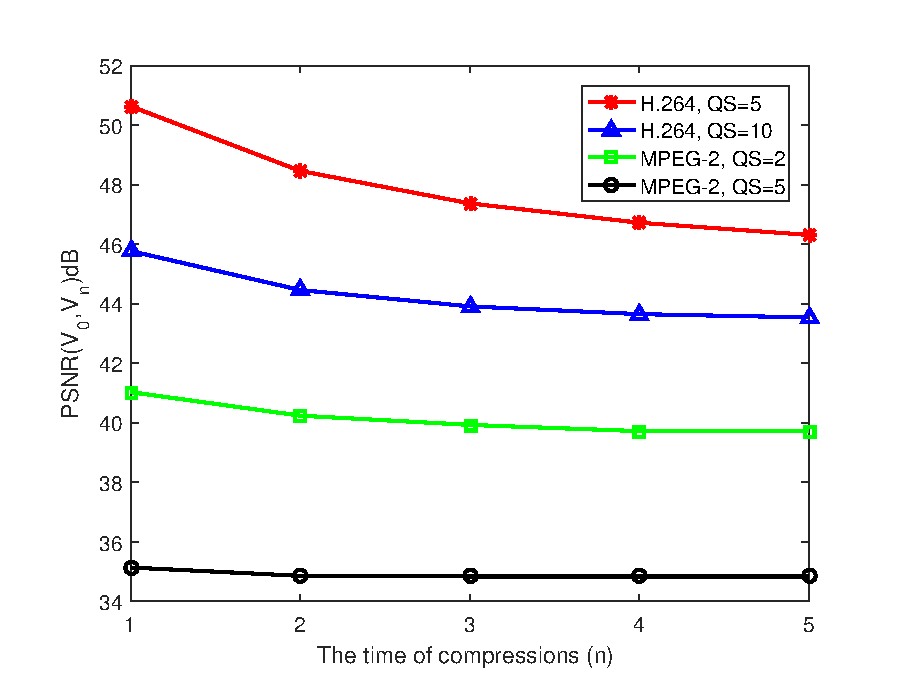
\includegraphics[width=0.40\textwidth,height=5.1cm]{psnr.eps}
		\label{fig:ipmbm}
	}
	\caption{Variation of video quality after continuous recompressions with the same coding parameters.
	}
	\label{fig:psnr}
\end{figure}

\begin{figure*}[ht!]
	\centering
	\subfigure[]{
		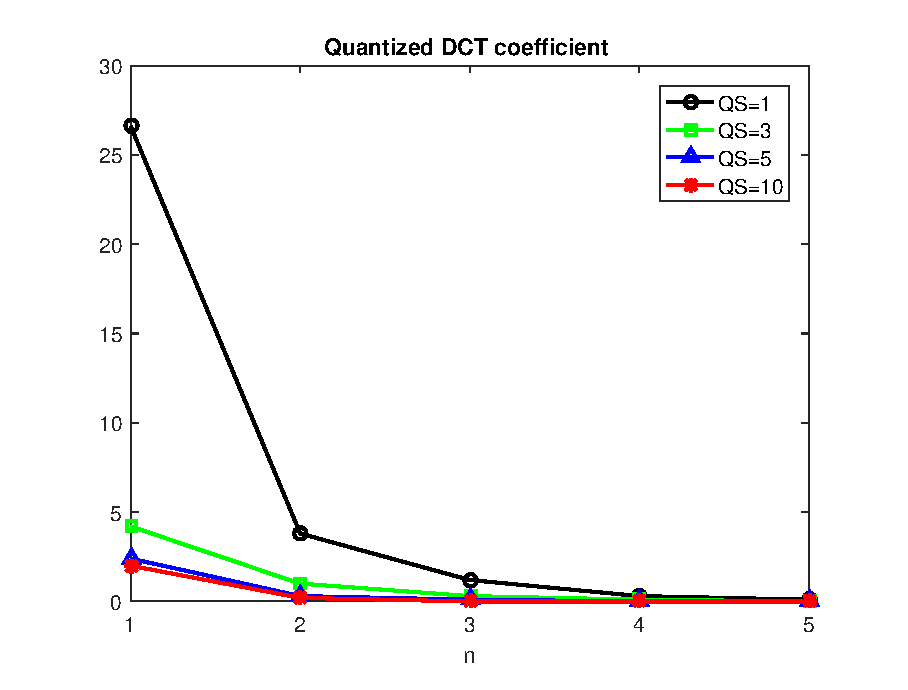
\includegraphics[width=0.45\textwidth,height=5.4cm]{sec2_dct.eps}
		\label{fig:dct}
	}
	\subfigure[]{
		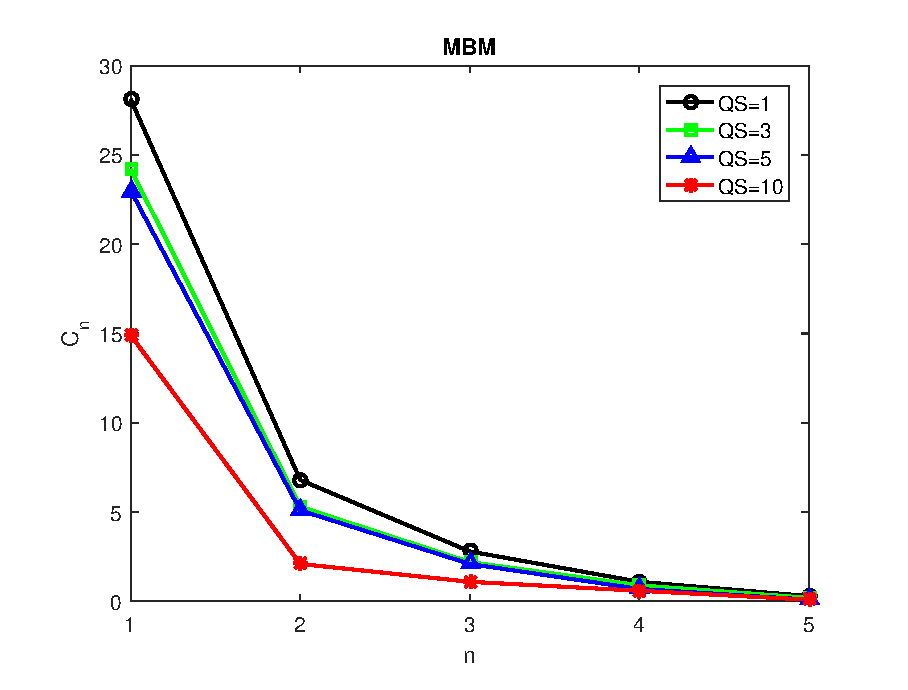
\includegraphics[width=0.45\textwidth,height=5.4cm]{sec2_mbm.eps}
		\label{fig:mbm}
	}
	\caption{(a) Variation tendency of the number of altered quantized DCT
		coefficients between $n$th compression and $(n+1)$th compression per I-frame. 
		(b) Variation tendency of the number of macroblocks with unstable MBM between $n$th compression and $(n+1)$th compression per P-frame ($C_n$).
		}
	\label{fig:statistics}
\end{figure*}


\section{Analysis of Quality Degradation Mechanism after Recompression}

In this section, an example of video quality degradation after recompressions is first presented. Then, quality degradation mechanisms after recompression are analyzed for different video coding standards, including MPEG family and H.264. The encoding strategies, such as motion estimation method, macroblock decision algorithm and so on, are assumed to be unchanged during continuous recompression processes.

\subsection{Variation of video quality after continuous recompressions}

An example is provided to illustrate how video quality changes after continuous recompressions with the same coding parameters. The YUV sequence ``container'' (CIF) in Appendix is selected as the raw video $V_0$. $V_0$ is encoded by the codec $c_0$ using quality scale ($QS$) $q_0$ to generate $V_1$. Decode $V_1$ to YUV file $Y_1$. Then conduct recompression on this file several times with the same coding parameters. Finally, several recompressed videos $V_n$ are obtained ($n=1,2...,5$). The average PSNRs (peak signal-to-noise ratio) between the raw video $V_0$ and recompressed videos $V_n$ are computed as the full-reference video quality metric. Only luminance components are considered to calculate PSNR. As shown in Fig. \ref{fig:psnr}, it can be observed that video quality tends to become nearly unchanged after multiple recompressions due to continuous degradation, which can be formally expressed as:
\begin{equation}
\text{PSNR}(V_0,V_{n+1}) =  \text{PSNR}(V_0,V_{n}) - \Delta \text{PSNR}
\label{psnr}
\end{equation}
where $\Delta \text{PSNR}$ is the quality degradation caused by recompression operation. Since single compressed videos ($V_1$) and double compressed videos ($V_2$) undergo once and twice compression respectively, they suffer different degrees of quality degradation. This property can be used to expose double compression with the same coding parameters. However, for larger $QS$ and traditional video encoders (e.g. $c_0=\text{MPEG-2}$, $q_0=5$), the difference between PSNR($V_0,V_1$) and PSNR($V_0,V_2$), namely $\Delta \text{PSNR}$, is slight and it is hard to discriminate the single and double compressed videos. To provide more robust and efficient measurement of quality degradation, we will analyze the degradation mechanisms after recompression in different compression standards and compression qualities. Obviously, unchanged video quality is roughly equivalent to unchanged states of video data in compression domain after recompression. In following subsections, we will study the relationship between the variation tendency of several video data and the degree of quality degradation. 


\begin{table}
	\setlength{\abovecaptionskip}{0.cm}
	\setlength{\belowcaptionskip}{-0.cm}
	\small
	\centering
	\caption{\label{notation}Notation}
		\begin{tabular}{ l p{7.5cm} }
			$\mathbf{D}_n$ &quantized DCT coefficients, $\mathbf{D}_n\in \mathbb{Z}^{8\times8}$\\
			$\mathbf{E}_n$ &error block, $\mathbf{E}_n\in \mathbb{R}^{8\times8}$ \\
			$\mathbf{R}_n$ &quantized DCT coefficients of an error block, $\mathbf{R}_n\in \mathbb{Z}^{8\times8}$ \\
			$\mathbf{B}_n$ &pixel coefficients, $\mathbf{B}_n\in \mathbb{N}^{8\times8}$ \\
			$\mathbf{\hat{B}}_n$ &reconstructed pixel coefficients, $\mathbf{\hat{B}}_n\in \mathbb{N}^{8\times8}$ \\
			$\mathbf{P}_n$ &quantized DCT coefficients of prediction residual, $\mathbf{P}_n\in \mathbb{Z}^{8\times8}$ \\
			$\mathbf{Q}$ &quantization matrix, $\mathbf{Q}\in \mathbb{N}^{8\times8}$\\
			$n$ &the number of compression operations applied to the input sequence\\
		\end{tabular}
\end{table}

\subsection{The quality degradation mechanism in MPEG compression}
The quality degradation can be classified into two categories, including degradation in the intra-coding process and degradation in the inter-coding process. Since the encoding process is not constrained by the video compression standard, the MPEG-2 codec in the library ``libavcodec'' through FFmpeg\cite{FFmpeg} is used as an example to illustrate the compression and decompression procedures. We only consider luminance components in the theoretical analysis.

\subsubsection{Degradation in the intra-coding process \label{degrad-intra}}
In the MPEG-2 standard, the intra-coding process is similar to JPEG compression. Concretely, raw frames are first partitioned into non-overlapping blocks (e.g. macroblocks of $16\times16$ pixels). Then, the DCT transformation and quantization process are conducted on each $8\times8$ sub-block individually. There are three kinds of errors contributing to quality degradation in the intra-coding process. The first one, namely the quantization error, is caused by mapping the float value of the quantized DCT coefficient to its nearest integer value. It is the principal source of information loss in video compression. 

The second and third degradation errors both exist in the decompression process, namely the rounding error and the truncation error. The rounding error is defined as the difference between a float IDCT coefficient whose value is within $[0,255]$ and its rounded integer. The truncation error is defined as the difference between a float IDCT coefficient whose value exceeds $[0,255]$ and its truncated integer (e.g. $0$ or $255$). According to the implementation in MPEG-2 codec libavcodec library \cite{FFmpeg}, the entire intra-coding process in $(n+1)$th compression can be expressed as follows:
\begin{equation}
\mathbf{D}_{n+1}= \left[\frac{DCT(RT(IDCT(\mathbf{D}_n\times\mathbf{Q}\times QS)))}{\mathbf{Q}\times QS}\right] 
\label{entire-intra}
\end{equation}
where the subscript $n$ denotes the times of MPEG compression; $DCT(\cdot)$ and $IDCT(\cdot)$ represent $8\times8$ discrete cosine transform and inverse discrete cosine transform separately; $\mathbf{Q}$ denotes the default intra-quantization matrix; $RT(\cdot)$ denotes rounding and truncating a real number to integer in the range of [0, 255]; $[\cdot]$ denotes rounding operation and all the basic arithmetic operation is component-wise. The error block ($\mathbf{E}_n$) after the inverse discrete cosine transform is defined as:

\begin{equation}
\mathbf{E}_n= RT(IDCT(\mathbf{D}_n\times\mathbf{Q}\times QS))-IDCT(\mathbf{D}_n\times\mathbf{Q}\times QS)
\label{error-define}
\end{equation}

If the quality of a video is very high, the quality degradation caused by quantization and rounding/truncating operation are comparable \cite{sorial1998degradation}. To analyze the impact of rounding/truncating operation, the quantization process in Eq. (\ref{entire-intra}) is rewritten as follows:
\begin{equation}
\begin{aligned}
\mathbf{D}_{n+1} & =\left[\frac{DCT(IDCT(\mathbf{D}_n\times\mathbf{Q}\times QS)+\mathbf{E}_n)}{\mathbf{Q}\times QS}\right]\\
& = \mathbf{D}_n + \left[\frac{DCT(\mathbf{E}_n)}{\mathbf{Q}\times QS}\right]\\
& = \mathbf{D}_n + \mathbf{R}_n
\label{intra-n+1}
\end{aligned}
\end{equation}


It can be found that the magnitude of quality degradation after recompression in I-frames, namely $\mathbf{R}_n$, is related to the setting of quality scale ($QS$) and quantization matrix $\mathbf{Q}$. If $\mathbf{R}_n$ is equal to a zero matrix, the elements in $\mathbf{D}_n$ will no longer change in its next compression \cite{yang2014effective}. We call this kind of blocks as stable block. $\mathbf{R}_n$ is more likely to become zero with the time of recompressions increasing. It infers that statistics of rounding and truncation errors ($\mathbf{E}_n$) are distinguishing between single and double compressed I-frames, when the value of $QS$ is small. For a larger value of $QS$, $\mathbf{R}_n$ is more likely to become zero instantly after single compression. It means most of the blocks in single compressed I-frames are stable blocks when the quantization step ($\mathbf{Q}\times QS$) is large. Since the quality degradation ($\mathbf{R}_n$) is the difference between $\mathbf{D}_n$ and $\mathbf{D}_{n+1}$, the variation tendency of quantized DCT coefficients after recompression is analyzed for different $QS$. As shown in Fig. \ref{fig:dct}, each point denotes the average number of altered quantized DCT coefficients between $n$th compression and $(n+1)$th compression per I-frame for a specific $QS$. It is calculated on 132 raw video clips, which are illustrated detailedly in section \ref{dataset_video}. For a small value of $QS$ (e.g. $QS$=1), the amount of altered quantized DCT coefficients after recompression varied dramatically between single ($n=1$) and double ($n=2$) compressed I-frames. For a large value of $QS$ (e.g. $QS$=5), it is obvious that the quantized DCT coefficients become almost unchanged after single compression. This observation confirms the theoretical analysis mentioned above. Rounding and truncation errors are discriminating between single compressed and double compressed I-frames in high-quality videos.  


\subsubsection{Degradation in the inter-coding process \label{degrad-inter}}
To reduce temporal redundancy of video contents, the MPEG-2 standard applies motion estimation and motion compensation techniques in their hybrid video coding framework. Motion estimation is the process to find out the transformation from the current frame to its reference frame. For simplicity, we do not consider B-frames in this work. The motion vector $(V_x, V_y)$ is the optimized displacement which minimizes the difference between the current block and its predicted block. It can be formally expressed as:
\begin{equation}
\begin{aligned}
(V_x, V_y) & = \mathop{\arg min}_{V_x, V_y}f_M\left(\mathbf{B}_n^{(i,j,t)}, \mathbf{\hat{B}}_n^{(i+V_x, j+V_y,t-\Delta t)}\right)
\label{motion-comp}
\end{aligned}
\end{equation}
where $f_M(\cdot,\cdot)$ denotes the measurement of difference between two blocks, e.g. sum of absolute differences (SAD); $\mathbf{B}_n^{(i,j,t)}$ denotes a block in the current frame ($t$th frame) whose up-left corner locates at $(i,j)$ while $\mathbf{\hat{B}}_n^{(i+V_x, j+V_y,t-\Delta t)}$ denotes its predicted block reconstructed in the reference frame; $\Delta t$ indicates the temporal distance between the current frame and its reference frame, which is set to 1 by default in the MPEG-2 codec. The range of motion vector components $V_x$ and $V_y$ is followed with the default settings in FFmpeg\cite{FFmpeg}. Please note the rate-distortion optimization algorithms for motion estimation and mode decision are assumed to be identical during the recompression process. Based on this constraint, the potential alternation introduced by different rate-distortion optimization algorithms can be neglected to simplify the problem formulation.

Similar to the intra-coding process, the primary source of information loss in motion compensation is caused by the quantization process of prediction residuals.
\begin{equation}
\begin{aligned}
\mathbf{P}_n = \left[ \frac{DCT(\mathbf{B}_n -\mathbf{\hat{B}}_n)}{\mathbf{Q}\times QS}\right]
\label{resi-quan}
\end{aligned}
\end{equation}
where $\mathbf{B}_n$ and $\mathbf{\hat{B}}_n$ denotes the current block and its reconstructed reference block in the $n$th compression respectively. Since the current block ($\mathbf{B}_n$) is the combination of reconstructed prediction residuals from $\mathbf{P_n}$ and the reconstructed reference block ($\mathbf{\hat{B}_n}$), elements in $\mathbf{B}_n$ cannot become unchanged before $\mathbf{\hat{B}}_n$ converges to a stable state. Besides, the compression error of the first frame (I-frame) in each GOP can be propagated to its following P-frames by motion compensation. It means the quality of P-frames is more difficult to become unchanged after continuous recompressions than I-frames even with more severe quantization. 

\begin{figure*}[ht!]
	\centering
	\subfigure[]{
		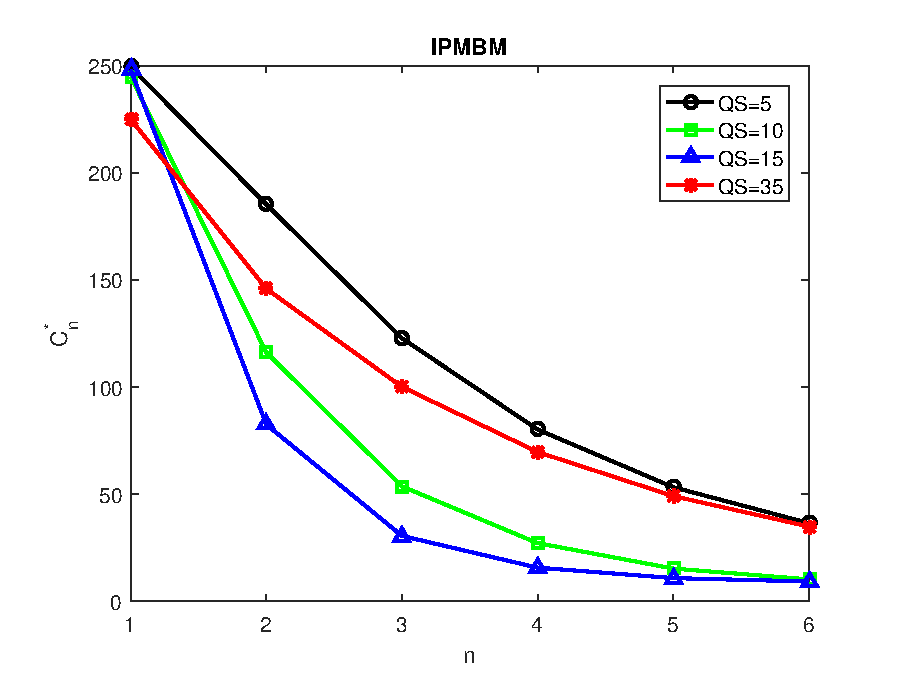
\includegraphics[width=0.45\textwidth,height=5.4cm]{sec2_ipmbm.eps}
		\label{fig:ipmbm2}
	}
	\subfigure[]{
		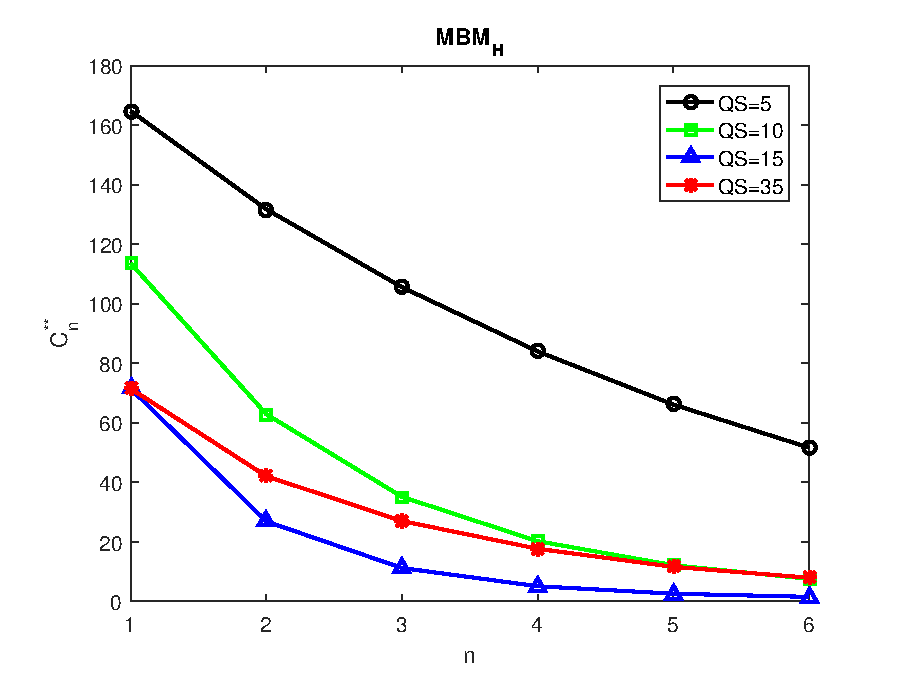
\includegraphics[width=0.45\textwidth,height=5.4cm]{sec2_mbmh.eps}
		\label{fig:mbmh}
	}
	\caption{(a) Variation tendency of the number of macroblocks with unstable IPMBM between $n$th compression and $(n+1)$th compression per I-frame. 
		(b) Variation tendency of the number of macroblocks with unstable $\text{MBM}_\text{H}$ between $n$th compression and $(n+1)$th compression per P-frame.
	}
	\label{fig:statistics_h264}
\end{figure*}
 
In our previous work, we defined macroblock mode (MBM) as the state of macroblocks in P-frames. The MBM of a macroblock is defined as follows:
\begin{equation}
MBM(\mathbf{M}) = \{M_{type},M_{mv}\} \label{mbm-define}
\end{equation}
where $\mathbf{M}$ denotes a macroblock; $M_{type}$ denotes the macroblock type, $M_{mv}$ denotes the motion vectors of $\mathbf{M}$. $M_{type}\in \{\text{I-MB,P-MB,S-MB}\}$ and $M_{mv}=\{(V_x,V_y)|V_x,V_y\in \mathbb{Z}\}$. If $M_{type}$ is I-MB or S-MB, $M_{mv}$ of this macroblock is set to $(0,0)$. Two macroblocks have the same macroblock mode only when they have identical macroblock type and motion vectors. If a macroblock at the same position has an identical macroblock mode between $n$th compression and $(n+1)$th compression, this macroblock is considered as temporarily stable in $n$th compression. Otherwise, this macroblock has unstable MBM. The average number of macroblocks with unstable MBM between $n$th compression and $(n+1)$th compression per P-frame, namely $C_n$, is formulated as:

\begin{equation}
C_n = \frac{1}{T_P}\sum_{t=1}^{T_P}\sum_{i=1}^{H}\sum_{j=1}^{W}I(\mathbf{M}_n^{(i,j,t)},\mathbf{M}_{n+1}^{(i,j,t)}) \label{ave-mode}
\end{equation}
where $T_P$ denotes the total number of P-frames in the input video; $H$ and $W$ denote the vertical and horizontal maximum index of macroblocks respectively; $\mathbf{M}_n^{(i,j,t)}$ denotes the macroblock in $n$th compression ($n\in\{1,2,...\}$), which locates at $(i,j)$ of the $t$th P-frames. The indicator function $I(\cdot,\cdot)$ in Eq. (\ref{ave-mode}) is defined as:

\begin{equation}
I(\mathbf{M}_1,\mathbf{M}_2) =
\begin{cases}
1, & MBM(\mathbf{M}_1) \ne MBM(\mathbf{M}_2) \\
0, & MBM(\mathbf{M}_1) = MBM(\mathbf{M}_2)
\end{cases}
\label{indicator}
\end{equation}
where $\mathbf{M}_1$ and $\mathbf{M}_2$ denote two macroblocks.

The average number of macroblocks with unstable MBM per P-frame ($C_n$) on 132 raw video clips is presented in Fig. \ref{fig:mbm}. Compared with the convergent tendency of quantized DCT coefficients, MBM in P-frames is harder to become unchanged after single compression with large values of $QS$. The average number of macroblocks with unstable MBM between single compressed ($n=1$) and double compressed ($n=2$) P-frames has the distinct difference. It demonstrates that the convergence of inter-coding data's state, such as MBM, is more robust to discriminate single and double compressed videos in low-quality. Due to the similar coding framework and techniques used in MPEG-4 standard, similar properties of quality degradation can be obtained in MPEG-4 videos.




\subsection{The degradation mechanism in H.264 standard\label{degrad_h264}}
In the last decade, H.264 has become the most commonly used video compression standard for data transmission on the Internet and data storage of mobile devices. Similar to the MPEG compression standards (e.g. MPEG-2 and MPEG-4), it applies hybrid video coding scheme to reduce the spatial and temporal redundancy of raw video files. Different from traditional standards, H.264 introduces several advanced techniques to improve the coding efficiency and visual quality, such as intra-prediction mode and in-loop deblocking filter. 



\subsubsection{Degradation in the intra-coding process \label{degrad-intra_h264}}
In the intra-coding process, a current block selects a prediction block based on reconstructed blocks to calculate the corresponding residual block. Two types of prediction modes can be selected to encode luminance components of macroblocks in I-frames, namely $\text{Intra}\_\text{4x4}$ and $\text{Intra}\_\text{16x16}$. Then, the transformation and quantization process are conducted on residual blocks. Although quantization errors are still the main source of information loss, the intra-coding process of H.264 videos is much more complicated than MPEG videos due to the intra-prediction technique.

Instead of providing a complicated mathematical model, we utilize the variation tendency of video data after recompression to analyze the degree of quality degradation in H.264 videos. It is inspired by the properties of quality degradation mechanisms on MPEG videos. In this work, intra-prediction macroblock mode (IPMBM) is proposed to describe the state of a macroblock in I-frames of H.264 videos. It contains two kinds of significant video data in the compression domain, including macroblock type and the prediction mode of each sub-block, which is formally expressed as:
 \begin{equation}
 IPMBM(\mathbf{M}) = \{M_{type},M_{pre}\}\label{ipmbm-define}
 \end{equation}
where $\mathbf{M}$ denotes a macroblock, $M_{type}$ denotes the macroblock type, $M_{pre}$ denotes the information of intra-prediction mode \cite{wiegand2003overview}.
 
 \begin{itemize}    
 	\item If $M_{type}$ is $\text{Intra}\_\text{16x16}$, IPMBM is expressed as
 	\begin{equation}
 	IPMBM(\mathbf{M}) = \{\text{Intra}\_\text{16x16},M_{pre}\}
 	\end{equation}
 	where $M_{pre}$ denotes the intra prediction mode of a $16\times16$ sub-block and $ M_{pre} \in $\{Vertical, Horizontal, DC, Plane\}.
 	
 	\item If $M_{type}$ is $\text{Intra}\_\text{4x4}$, IPMBM is expressed as
 	\begin{equation}
 	\begin{aligned}
 	&IPMBM(\mathbf{M}) = \{ \text{Intra}\_\text{4x4},\{M_{pre_1},M_{pre_2}...,M_{pre_{16}}\}\}\\
 	\end{aligned}
 	\end{equation}
 	where $M_{pre_i}$ denotes the intra-prediction mode of the $i$th 4$\times$4 sub-block. $M_{pre_i} \in$ \{Vertical, Horizontal, DC,  Diagonal-Down-Left, Diagonal-Down-Right, Vertical-Right, Horizontal-Down, Vertical-Left, Horizontal-UP\}. 
 \end{itemize}	
 
Two macroblocks belong to the same IPMBM only when they have same macroblock type and intra-prediction modes. If a macroblock at a fixed position has different IPMBMs between $n$th compression and $(n+1)$th compression, this macroblock has unstable IPMBM in $n$th compression. The average number of macroblocks with unstable IPMBM per I-frame ($C^*_n$) is calculated in the same way as $C_n$ in Eq. (\ref{ave-mode}), except that $T_P$ is replaced by $T_I$ in Eq. (\ref{ave-mode}) and $MBM(\cdot)$ is replaced by $IPMBM(\cdot)$ in Eq. (\ref{indicator}). $T_I$ denotes the number of I-frames in the input video. The variation tendency of $C^*_n$ for different $QS$s\footnote{For the sake of simplicity, $QS$ is equivalent to $QP$ for H.264-based encoders.} is calculated on 132 raw video clips as shown in Fig. \ref{fig:ipmbm2}. In each curve, the value of $C^*_n$ decreases monotonously with the value of $n$ increasing. It infers the state of video data in compression domain (equivalent to video quality) tends to become unchanged after continuous recompressions. The distinct gap between $C^*_1$ and $C^*_2$ in each curve indicates that the number of macroblocks with unstable IPMBM can be used to discriminate different degrees of quality degradation between single and double compressed I-frames. Interestingly, unlike MPEG videos, IPMBMs perform slower convergent speed to the unchanged state for several larger $QS$s (e.g. $QS=35$). It is due to the complex intra-prediction mode decision strategy and error propagation through the intra-prediction process. 
 

\subsubsection{Degradation in the inter-coding process \label{degrad-inter_h264}}
In the inter-coding process, several advanced techniques make the properties of quality degradation on H.264 videos more complicated than MPEG videos, such as variable block-size prediction and in-loop deblocking filters. It is too intricate to describe the inter-coding process on H.264 videos using a mathematical model. To measure the degree of quality degradation, the concept of MBM in MPEG videos is extended to H.264 videos. The macroblock mode $\text{MBM}_{\text{H}}$ in P-frames of H.264 videos is defined as: 
\begin{equation}
\begin{aligned}
&MBM_{H}(\mathbf{M}) = \{M_{type},\{M_{mv_1},M_{mv_2}...,M_{mv_{16}}\}\},\\
& \begin{cases}
M_{type}\in&\{\text{Inter}\_\text{16x16},\text{Inter}\_\text{16x8},\text{Inter}\_\text{8x16},\text{Inter}\_\text{8x8},\\
&\text{P}\_\text{Skip},\text{Intra}\_\text{16x16},\text{Intra}\_\text{4x4}\} \\
M_{mv_i}=&\{(V_x,V_y)|V_x,V_y\in \mathbb{Z}\}
\end{cases}\\
\end{aligned}
\end{equation}
where $M_{mv_i}$ denotes the motion vector of the $i$th sub-block. If $M_{type}$ is $\text{Intra}\_\text{16x16},\text{Intra}\_\text{4x4}$ or $\text{P}\_\text{Skip}$, the motion vector of each sub-block in the corresponding macroblock is set to $(0, 0)$. 

 \begin{figure*}[ht!]
 	\centering
 	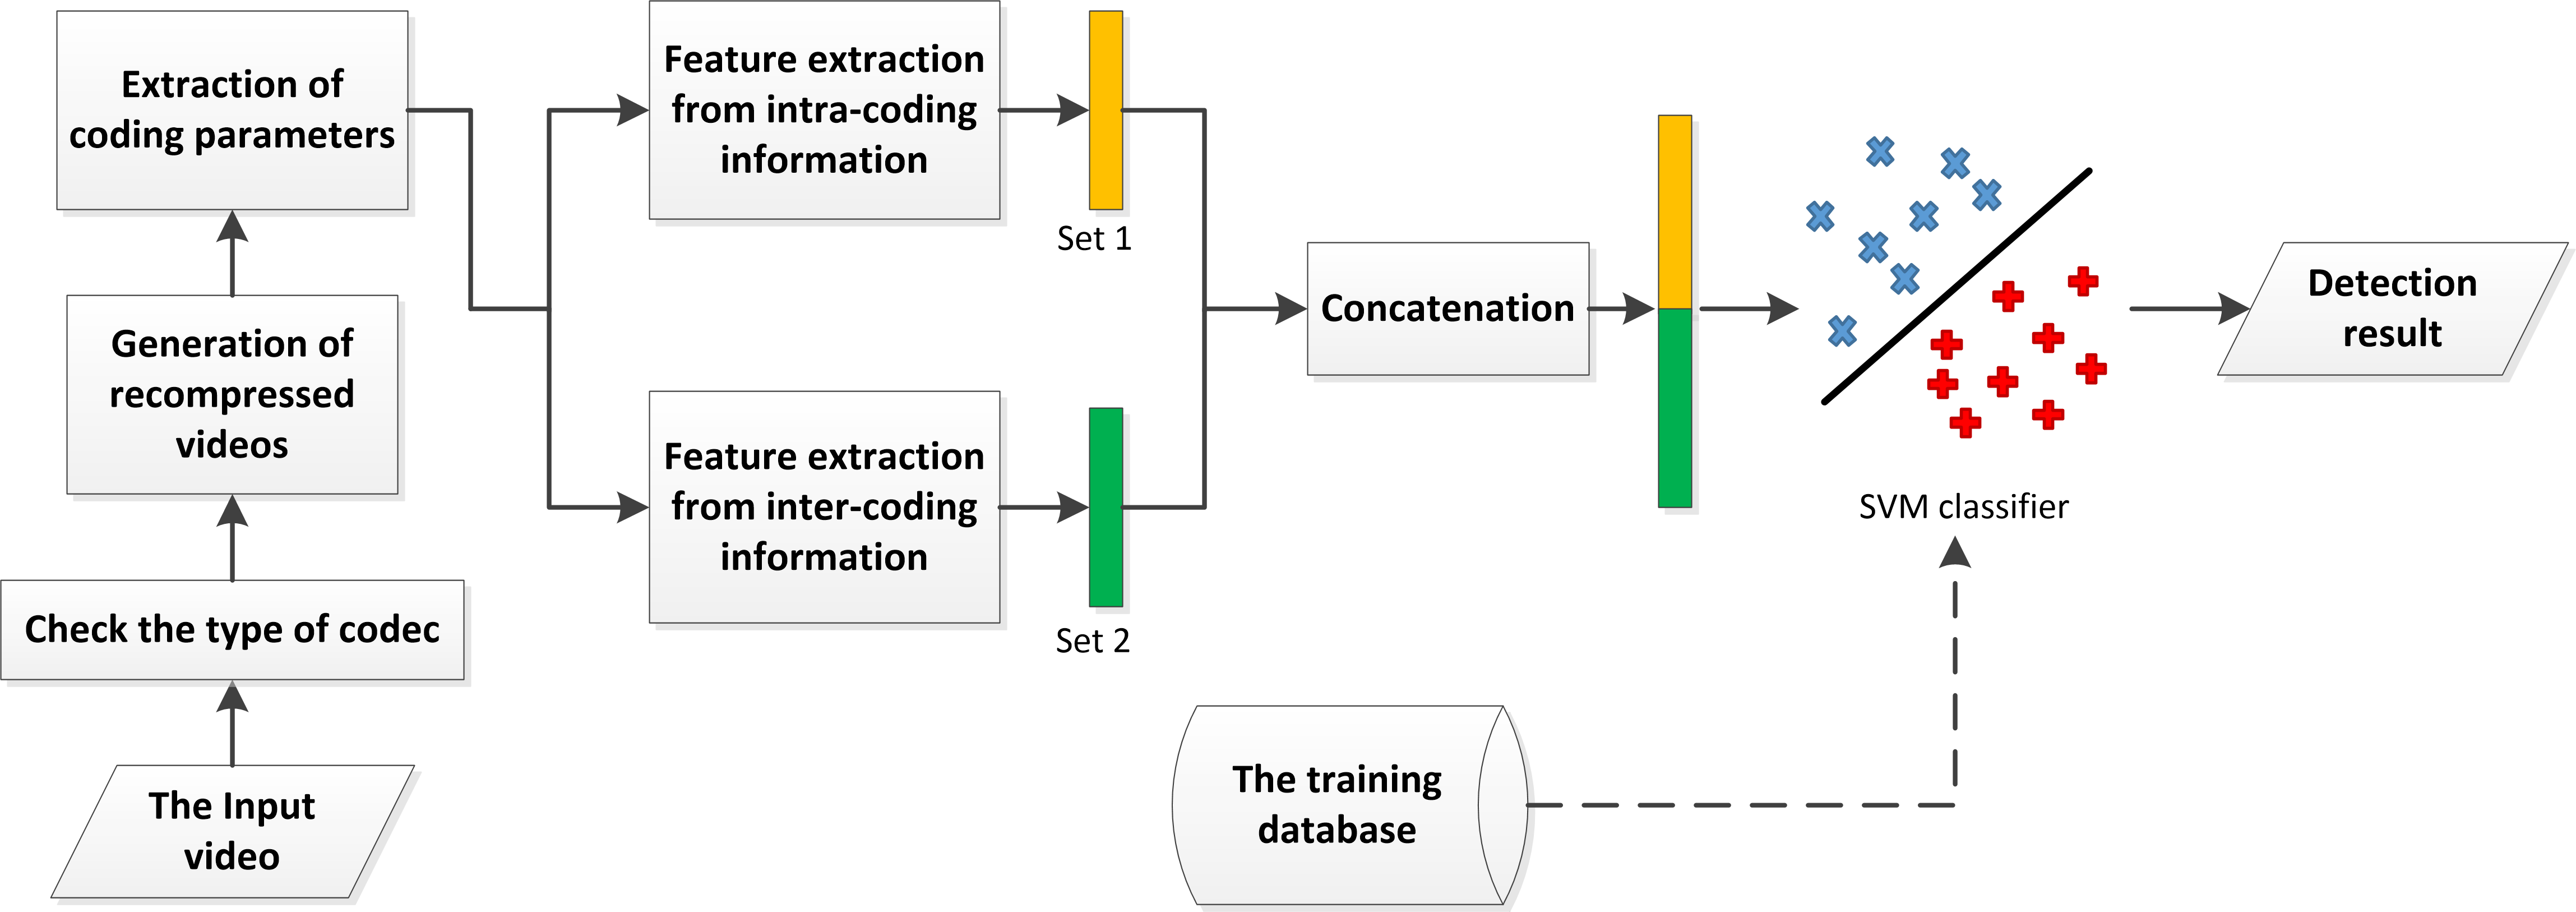
\includegraphics[width=0.81\textwidth,height=5cm]{detection_pipeline.png}
 	\caption{\label{Fig.framework}The framework of the proposed method}
 \end{figure*}

The average number of macroblocks with unstable $\text{MBM}_\text{H}$ per P-frame ($C^{**}_n$) is calculated in the same way as $C_n$ in Eq. (\ref{ave-mode}), except that $MBM(\cdot)$ is replaced by $MBM_H(\cdot)$ in Eq. (\ref{indicator}). To analyze the quality degradation properties in P-frames of H.264 videos, the variation tendency of $C^{**}_n$ for different $QS$s is provided in Fig. \ref{fig:mbmh}. Similar to MBM, all the curves in Fig. \ref{fig:mbmh} have monotonously decreasing tendency. It can be found that the convergent speed of $C^{**}_n$ first becomes faster and then slows down with the value of $QS$ increasing. It is because when a video is encoded with very low quality (e.g. $QS=$35) and then decoded, the in-loop deblocking filter will significantly alter pixel value of reference frames. This kind of alternation makes $\text{MBM}_\text{H}$ more difficult to converge to an unchanged state after continuous recompressions for a very large $QS$ in H.264 videos. Besides, for a specific $QS$, the gap between $C^{**}_1$ and $C^{**}_2$ is smaller than the difference between $C^{*}_1$ and $C^{*}_2$ in Fig. \ref{fig:ipmbm2}. It infers the discrimination capability between single and double compression of $\text{MBM}_\text{H}$ is worse than IPMBM. This property will be verified in section \ref{evaluation_h264}. 



\section{The proposed method}
Based on the theoretical analysis, we found that the quality degradation mechanisms can be used to detect double compression and have diverse properties for different compression qualities. To provide more robust forensics tools for double compression detection, we use a concatenation fusion strategy combining features extracted from the intra-coding process and the inter-coding process. Due to different coding techniques used in the MPEG standards and the H.264 standard, two sorts of codec-specific algorithms are proposed, called as double MPEG compression detection method based on degradation mechanism analysis (referred to as MPEG-DM method) and double H.264 compression detection method based on degradation mechanism analysis (referred to as H264-DM method) respectively. As shown in Fig. \ref{Fig.framework}, the pipelines of those two approaches are very similar. However, the details of each function block in Fig. \ref{Fig.framework} are different between MPEG-DM method and H264-DM method. In the feature extraction process, we only consider luminance components. 


\subsection{MPEG-DM method}
For MPEG videos, the classification feature is generated by concatenating features extracted from intra-coding data ($f_{intra\_\text{M}}$) and inter-coding data ($f_{inter\_\text{M}}$).


\subsubsection{Features extracted from intra-coding data in MPEG videos ($f_{intra\_\text{M}}$)}
As mentioned in section \ref{degrad-intra}, the rounding and truncation errors in Eq. (\ref{error-define}) play a dominant role in quality degradation after recompression on high-quality videos. Same as the definition in \cite{yang2014effective}, a rounding error block $\mathbf{E}^r$ is an error block whose elements all belong to the range [-0.5, 0.5] while a truncation error block $\mathbf{E}^t$ is an error block of which at least one element exceeds the range [-0.5, 0.5]. In this work, we only consider unstable error blocks which contain at least one non-zero element. To describe the quality degradation caused by rounding and truncation errors in I-frames of MPEG videos, we selected a part of statistical features from \cite{yang2014effective} and modified them to construct our detection features for the intra-coding process ($f_{intra\_\text{M}}$) considering the balance between computational cost and detection effectiveness. It is extracted from rounding error blocks and truncation error blocks respectively. For rounding error blocks, a 4-D feature is obtained as follows: 

\begin{enumerate}	
	\item For an input video which contains $T_I$ I-frames, the rounding error blocks in each I-frame are calculated.
	\item The first dimension is the average number of rounding error blocks per I-frame.
	\begin{equation}
	\overline{L}^r=\frac{\sum_{t=1}^{T_I} L_t^r}{T_I} \label{mean-r}
	\end{equation}
	where $L_t^r$ means the number of rounding error blocks in $t$th I-frame.
	\item The second dimension is the maximum value of elements in rounding error blocks over all I-frames.
	\begin{equation}
	\begin{aligned}
	E^r_{max} = &\max |\mathbf{E}^r_\emph{k}(i,j)|\\\
	&k\in\{1,2,...,L^r\};i,j\in\{0,1,...,7\}%,j\in\{0,1,...,7\}
	\end{aligned}
	\end{equation}
	where $L^r$ denotes the total number of rounding error blocks in I-frames, namely $L^r = \sum_{t=1}^{T_I} L_t^r$. 
	\item The third dimension is the average value of all elements in rounding error blocks $\mathbf{E}^r$ of I-frames.
	\begin{equation}
    E^r_{avg} = \frac{\sum\limits^{L^r}_{k=1}\sum\limits^7_{i=0}\sum\limits^7_{j=0}|\mathbf{E}^r_k(i,j)|}{64L^r}
	\end{equation}	
	\item The last dimension is the variation value of all elements in rounding error blocks $\mathbf{E}^r$ of I-frames.
	\begin{equation}
	E^r_{var} = \frac{\sum\limits^{L^r}_{k=1}\sum\limits^7_{i=0}\sum\limits^7_{j=0}\left(|\mathbf{E}^r_k(i,j)|-E^r_{avg}\right)^2}{64L^r}\label{var-r}
	\end{equation}
\end{enumerate}

 For truncation error blocks, the feature extraction process is similar, where $\mathbf{E}^r_\emph{k}$ in Eq. (\ref{mean-r}) - (\ref{var-r}) is replaced by $\mathbf{E}^t_\emph{k}$. Thus, another 4-D feature vector can be obtained, namely $\left[\overline{L}^t,E^t_{max},E^t_{avg},E^t_{var}\right]$. Then, features extracted from rounding and truncation error blocks are concatenated as the 8-D feature of intra-coding data $f_{intra\_\text{M}} =$$ \left[\overline{L}^r,E^r_{max},E^r_{avg},E^r_{var},\overline{L}^t,E^t_{max},E^t_{avg},E^t_{var}\right]$.
 
 
 
\subsubsection{Features extracted from inter-coding data in MPEG videos ($f_{inter\_\text{M}}$)\label{inter_MBM}}
 In our previous work \cite{chen2016detecting}, the convergent properties of inter-coding data after recompression are utilized to construct macroblock mode (MBM) feature, which is also called as $f_{inter\_\text{M}}$ hereinafter. The definition of MBM is presented in Eq. (\ref{mbm-define}). The average number of macroblocks with unstable MBM per P-frame ($C_n$) is calculated using the formulation in Eq. (\ref{ave-mode}). The extraction process of $f_{inter\_\text{M}}$ is summarized as the following steps:

\begin{enumerate}
	
 \item Decode the input video $V$ to YUV file $Y_1$ and extract macroblock mode information $\mathcal{M}_1$ of all
 macroblocks in $V$. 
 \item Recompress the YUV file $Y_n$ to video $V_n$ with
 the same coding parameters, $n = 1,2,...,K$. Then decode $V_n$ to YUV file $Y_{n+1}$ and extract its macroblock mode information $\mathcal{M}_{n+1}$ at the same time.
 \item Repeat Step 2) for $K$ times. Then count the average number of macroblocks with unstable MBM ($C_n$) between
 $\mathcal{M}_n$ and $\mathcal{M}_{n+1}$ using Eq. (\ref{ave-mode}) and Eq. (\ref{indicator}). Considering the computational efficiency and detection capability, $K$ is set as 5 in this work.
 
 \item Consequently, 5-D feature $f_{inter\_\text{M}}=[C_1,C_2,C_3,C_4,$ $C_5 ]$ is extracted from P-frames.
\end{enumerate}

 
After extracting $f_{intra\_\text{M}}$ and $f_{inter\_\text{M}}$, two sets of features are concatenated as the final 13-D detection feature of the input video, $f_{combine\_\text{M}} = [f_{intra\_\text{M}}, f_{inter\_\text{M}}]$. Then, SVM is employed for classification using $f_{combine\_\text{M}}$ to obtain detection results.


\begin{figure*}[h]
	\label{dataset}
	\centering
	\subfigure[akiyo]{
		\label{Fig.sub.3}
		
\includegraphics[width=0.2\textwidth]{akiyo.png}}
	\hspace{0.15in}
	\subfigure[city]{
		\label{Fig.sub.4}
		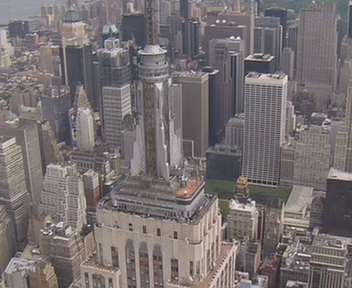
\includegraphics[width=0.2\textwidth]{city.png}}
	\hspace{0.15in}
	\subfigure[flower]{
		\label{Fig.sub.5}
		
\includegraphics[width=0.2\textwidth]{flower.png}}
	\subfigure[mobile]{
		\label{Fig.sub.6}
		
\includegraphics[width=0.2\textwidth]{mobile.png}}
	\caption{\label{Fig.example}Examples of YUV Sequences}
	\label{Fig.lable}
\end{figure*}

\begin{table*}
	\centering
	\caption{\label{encode-settings}The setting of video coding parameters}
	\begin{threeparttable}
		\begin{tabular}{ c c }
			\toprule
			& Parameter set  \\\midrule
			Codec&\{MPEG-2\tnote{1}, MPEG-4\tnote{1}, H.264\tnote{2}~\}\\\midrule
			Bit Rate Control Mode&\{Variant Bit Rate, Constant Bit Rate\}\\\midrule
			Compression Quality (VBR)&\{2,...,31\} for MPEG-2/4; \{1,2,...,52\} for H.264\\\midrule
			Compression Quality (CBR)&\{200, 300, ......, 900, 1000, 3000, 5000, 7000\}(kbps)\\
			\bottomrule
		\end{tabular}
		\begin{tablenotes}
			\footnotesize
			\item[1] MPEG-2/4 codec implemented in \emph{libavcodec} through \emph{FFmpeg}.
			\item[2] H264 codec implemented in \emph{libx264} through \emph{FFmpeg}.
		\end{tablenotes}
	\end{threeparttable}
\end{table*}

\subsection{H264-DM method}
Due to different advanced coding techniques used in the H.264 standard, it is required to design codec-specific features to detect double compression on H.264 videos. 


\subsubsection{Features extracted from intra-coding data in H.264 videos ($f_{intra\_\text{H}}$) \label{h264-ipmbm}}
Intra-prediction technique of the H.264 standard is a significant improvement in the intra-coding process compared with MPEG standards. The feature $f_{intra\_\text{M}}$ based on the previous intra-coding pipeline cannot be applied to H.264 videos directly. According to the observation in section \ref{degrad_h264}, the variation tendency of IPMBM after continuous recompressions can be used to measure the degree of quality degradation of I-frames in H.264 videos. Therefore, a detection feature based on intra-prediction macroblock mode (IPMBM) of I-frames is proposed. 

Similar to MBM in MPEG videos, if a macroblock located at a fixed position have different IPMBMs between $n$th compressed video and $(n+1)$th compressed video, this macroblock has unstable IPMBM in $n$th compression. The average number of macroblocks with unstable IPMBM between
$n$th compressed video and $(n+1)$th compressed video per I-frame ($C^*_n$) is used to generate $f_{intra\_\text{H}}$. The feature extraction process is identical to $f_{inter\_\text{M}}$ shown in Section \ref{inter_MBM}, except that $T_P$ is replaced by $T_I$ in Eq. (\ref{ave-mode}) and $MBM(\cdot)$ is replaced by $IPMBM(\cdot)$ in Eq. (\ref{indicator}). Consequently, 5-D feature $f_{intra\_\text{H}}=\left[C^*_1,C^*_2,C^*_3,C^*_4,C^*_5 \right]$ is extracted from I-frames.



\subsubsection{Features extracted from inter-coding data in H.264 videos ($f_{inter\_\text{H}}$) \label{h264-mbmh}}
In section \ref{degrad_h264}, macroblock mode of P-frames in H.264 videos ($\text{MBM}_\text{H}$) is proposed by extending the concept of MBM in $f_{inter\_\text{M}}$ based on unique coding structures in H.264 standard. The variation tendency of $\text{MBM}_\text{H}$ after continuous recompressions can be used to measure the degree of quality degradation of P-frames in H.264 videos. If a macroblock at a fixed position have different $\text{MBM}_\text{H}$s between $n$th compressed video and $(n+1)$th compressed video, this macroblock has unstable $\text{MBM}_\text{H}$ in $n$th compression. To construct $f_{inter\_\text{H}}$ feature for H.264 videos, the average number of macroblocks with unstable $\text{MBM}_\text{H}$ between $n$th compressed video and $(n+1)$th compressed video per P-frame ($C^{**}_n$) is calculated. The feature extraction process is the same as $f_{inter\_\text{M}}$ in Section \ref{inter_MBM}, except that $MBM(\cdot)$ is replaced by $MBM_H(\cdot)$ in Eq. (\ref{indicator}). Finally, 5-D feature $f_{inter\_\text{H}}=[C^{**}_1,C^{**}_2,$ $C^{**}_3,C^{**}_4,C^{**}_5]$ is extracted from P-frames. 

The features extracted in the intra-coding and inter-coding processes are concatenated as the final 10-D feature $f_{combine\_\text{H}}=[f_{intra\_\text{H}},f_{inter\_\text{H}}]$. Then it is fed to the SVM classifier to get final detection results.



\section{Experiments}

In this section, different compression qualities and video coding standards are first considered to evaluate the efficiency of the proposed method dealing with basic double compression cases. The proposed method is compared with sate-of-the-art algorithms, namely Huang's method for MPEG-2 videos \cite{huang2014detection} and Zhang's method for H.264 videos \cite{zhang2016detecting}. Next, the robustness of the proposed method under more realistic conditions is investigated, including more diverse video contents, various GOP sizes and different video spatial resolutions.


\subsection{Datasets\label{dataset_video}}
32 standard YUV sequences with CIF resolution (352$\times$288) are collected to construct the raw sequence dataset, referred to as dataset-A. More details about these sequences are presented in the Appendix, including the list of their names and the website address for downloading. The contents of these raw videos are diverse. Some of them are shown in Fig. \ref{Fig.example}. 


To increase sample quantity, for VBR mode, raw sequences are divided into non-overlapping video clips. Each video clip contains 100 frames. Sample generation and feature extraction are conducted on these video clips. For CBR mode, to prevent the rate control algorithm converging in an unreliable way with short-time clips as much as possible, compression operations of sample generation and feature extraction are conducted on the entire YUV sequence instead of raw video clips. Then, video-clip-wise samples (features) are obtained from every 100 encoded frames and their corresponding recompressed frames. If a YUV sequence includes more than 1000 frames, only the first 1000 frames are considered to generate samples in experiments. Consequently, 132 raw video clips can be generated based on this manner. The options of different parameters used in Section \ref{evaluation_mpeg2_all} to Section \ref{evaluation_h264} are reported in Table \ref{encode-settings}. The GOP size is fixed as 10 in all experiments, except for the experiment in Section \ref{evaluation_gop}. In Section \ref{evaluation_gop}, the robustness of the proposed method to different GOP sizes is evaluated. Besides, for simplicity, only baseline profile is considered in this work. From Section \ref{evaluation_mpeg2_all} to Section \ref{realistic}, in each experiment, the encoders used for generating training/testing video samples and extracting features are assumed to be configured with identical default settings of encoding strategies, including motion estimation, macroblock mode decision and so on. The limitation about this assumption will be discussed in Section \ref{diff_strategy}.

According to the parameter settings in Table \ref{encode-settings}, several subsets $S_{i,c,q}^m$ are constructed, where $i$ denotes the number of compression operations, $i\in \{1,2\}$; $c$ denotes the codec used in compression and decompression procedures; $m$ presents the bit rate control mode applied in encoding and $q$ denotes the compression quality (quality scale in VBR videos and average bit rate in CBR videos). On performance evaluation for a specific set of parameter settings (e.g. $c = c_0,q=q_0,m=m_0$), the single compressed video subset $S_{1,c_0,q_0}^{m_0}$ and its corresponding double compressed video subset $S_{2,c_0,q_0}^{m_0}$ are used to generate negative samples and positive samples respectively. Negative samples are randomly divided into two parts (1:1) for training and testing.
If a negative sample generated from the $d$th raw video clip $(d\in\{1,2,...,132\})$ is selected in training phase, the positive sample generated from the $d$th video clip should also be included in the training phase. 
In this manner, we can obtain the training set and the testing set. The binary classification is performed using an SVM classifier with RBF kernel. The optimized parameters $\gamma$ and $C$ are determined using grid search with 5-fold cross validation.

Detection accuracy is used as the criteria to evaluate the performance, which is defined as follows:
\begin{equation}
\frac{TN+TP}{N+P}\times 100 \% 
\end{equation}
where $N$ denotes the total number of negative samples, $P$ denotes the total number of positive samples, $TN$ denotes the number of correctly classified negative samples and $TP$ denotes the number of correctly classified positive samples. The detection accuracy reported in experiments is the average accuracy over 30 experiments by randomly selecting training data and testing data.



\subsection{Evaluation of performance on MPEG-2 videos\label{evaluation_mpeg2_all}}
In this section, the performance of MPEG-DM method is evaluated on MPEG-2 videos with VBR mode and CBR mode respectively. The dataset-A is used to generate training samples and testing samples. 

\subsubsection{VBR mode}
For VBR videos, the quality scale $QS$ in each macroblock is identical all the time. Therefore, VBR videos can keep the constant quality with various bit rates for different video contents. The properties of quantization errors in VBR videos are simpler than that in CBR videos. The performance is evaluated on each paired set of single compressed videos and double compressed videos, namely $S_{1,c,q}^{VBR}$ and $S_{2,c,q}^{VBR}$, where $c= \text{MPEG-2}$ and $q\in\{2,3,...,31\}$. The experimental results are shown in Fig. \ref{mpeg2-vbr}.

\begin{figure}[htbp!]
	\centering
	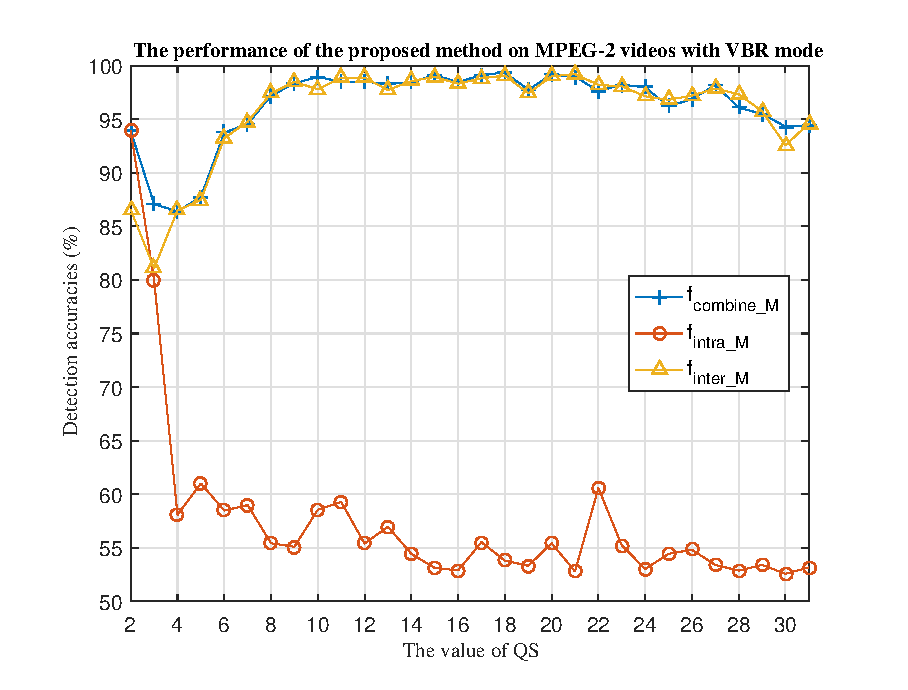
\includegraphics[width=0.5\textwidth]{MPEG2-VBR.eps}
	\caption{Evaluation of the performance on MPEG-2 videos with VBR mode}
	\label{mpeg2-vbr}
\end{figure}


According to results shown in Fig. \ref{mpeg2-vbr}, for high quality videos ($QS<4$), $f_{intra\_\text{M}}$ has competitive or even better accuracies than $f_{inter\_\text{M}}$. It is due to that the magnitude of rounding and truncation error is comparable to quantization error in this case. The rounding and truncation error plays a dominant role in quality degradation after recompression. However, with the value of $QS$ increasing, detection accuracies of $f_{intra\_\text{M}}$ drop down dramatically due to the severe quantization in the intra-coding process. The accuracies of $f_{intra\_\text{M}}$ are mostly lower than 60.00\% when $QS >4$. On the other hand, $f_{inter\_\text{M}}$ is much more robust than $f_{intra\_\text{M}}$ in both middle-quality and low-quality videos ($QS>20$). The concatenated feature $f_{combine\_\text{M}}$ achieves the higher average detection accuracy (96.29\%) than the results of $f_{inter\_\text{M}}$ (95.78\%) and $f_{intra\_\text{M}}$ (57.54\%). Note that $f_{intra\_\text{M}}$ may become noisy to deteriorate the classification performance slightly of $f_{combine\_\text{M}}$ when the video quality is very low.

\subsubsection{CBR mode \label{evaluation_mpeg2}}
Constant bit rate (CBR) is usually applied for streaming multimedia content on limited capacity channels. In this experiment, the performance of the proposed method and Huang's method \cite{huang2014detection} is evaluated on the CBR videos. In Huang's method, the input video $V$ ($b_0$ kbps) is first decompressed and then recompressed by $b_0$ kbps to generate a video $V'$. Next, the input video $V$ ($b_0$ kbps) is decompressed and then recompressed by another bit rate $(b_1 = b_0-\Delta b)$ kbps to generate a video $V''$, where $\Delta b$ is usually set as a small value in \cite{huang2014detection}. The number of altered quantized DCT coefficients between $V$ and $V'$ is called as $D_s$ while the number of altered quantized DCT coefficients between $V$ and $V''$ is called as $D_d$. The decision rule of double compression in Huang's method is as follows: If $D_s \geq D_d$, the input video is single compressed. And if $D_s < D_d$, the input video is double compressed. The average accuracy of Huang's method is obtained on the testing video samples over 30 experiments. $\Delta b$ is set to 20kbps when $b_0\in\{200,300,...,900\}$kbps and set to 100kbps when $b_0\in\{1000,3000,...,7000\}$kbps.

\begin{table}
	\centering
	\caption{\label{mpeg2-cbr}The detection accuracies of double compression on MPEG-2 videos with CBR mode (\%)}
	\begin{tabular}{ccccc}
		\toprule
		Bit rate \tnote{a}& $f_{combine\_\text{M}}$ & $f_{intra\_\text{M}}$ & $f_{inter\_\text{M}}$& Huang's  \\\midrule
		7000 &90.66   &\textbf{92.07}   &86.57   & 80.30\\
		5000 &89.37   &\textbf{90.68}   &84.37   & 81.24\\
		3000 &83.94    &\textbf{84.47}   &80.38  & 78.23\\\midrule
		1000 &\textbf{79.54}    &58.33   &79.47  & 77.46\\
		900 &\textbf{77.63}   &57.05   &75.15   & 75.18\\
		800 &\textbf{81.41}   &58.46   &78.99   & 75.26\\
		700 &\textbf{82.68}   &58.03   &80.56   & 76.33\\
		600 &\textbf{77.78}   &55.98   &76.84   & 74.45\\
		500 &\textbf{76.09}   &58.94   &73.18   & 67.89\\
		400 &\textbf{83.86}   &58.66   &82.32   & 65.71\\\midrule
		300 &\textbf{84.72}   &60.03   &81.49   & 63.24\\
		200 &\textbf{88.06}   &59.32   &82.25  & 63.68\\\midrule
		Average &\textbf{82.96}   &59.32   &80.13  & 73.24\\\bottomrule
	\end{tabular}
	\begin{tablenotes}
	\footnotesize
	\item[a] The unit of bit rate is \emph{kbps}
	\end{tablenotes}
\end{table}

According to the results in Table \ref{mpeg2-cbr}, our method $f_{combine\_\text{M}}$ obtains the highest average detection accuracy (82.96\%) compared to Huang's method (73.24\%). For very high-quality CBR videos (e.g. $3000$kbps $\leq b \leq 7000$kbps), $f_{intra\_\text{M}}$ outperforms $f_{combine\_\text{M}}$ and $f_{inter\_\text{M}}$. It infers that features based on statistical properties of rounding and truncation errors are more distinguishing between single compressed videos and double compressed videos when the quantization step is small. However, with the quality of videos becoming worse, $f_{combine\_\text{M}}$ and $f_{inter\_\text{M}}$ perform better detection capability. The accuracy of Huang's method drops rapidly with the value of bit rate decreasing, because the traces based on quantized DCT coefficients is easy to be destroyed by larger quantization steps.
%It is interesting that the performance of middle-quality (bit rate $\in\{500,600,...,1000\}(kbps)$) is worse than high-quality and low-quality videos. The insight behind this results is that the value of $QS$ for a macroblock in the same location varies distinctly during multiple recompressions , which depends on the rate control algorithm used in the codec. 
Note that, the proposed method achieves lower detection accuracies in CBR videos compared with the results in VBR videos. It is because the rate control algorithm chooses different quality scales to quantize different video contents, which aims at keeping bit rate constant over time. Therefore, different quality scales may be assigned to a macroblock in a fixed position during continuous recompression processes. This coding mechanism makes the property of quality degradation more complicated. It infers double compression detection in CBR videos is more challenging than that in VBR videos.



\subsection{Evaluation of performance on MPEG-4 videos\label{evaluation_mpeg4}}
Compared to MPEG-2, the MPEG-4 standard was mainly developed to achieve higher compression efficiency for mobile devices and online video transmission. To reduce the size of video data, several novel techniques are implemented in MPEG-4 part-2, such as shape coding and coefficient prediction. The performance of MPEG-DM method is evaluated on MPEG-4 videos in both VBR mode and CBR mode. The dataset-A is used to generate training samples and testing samples. The experimental results are presented in Fig. \ref{mpeg4-vbr} and Table \ref{mpeg4-cbr}.

\begin{figure}[htbp!]
	\centering
	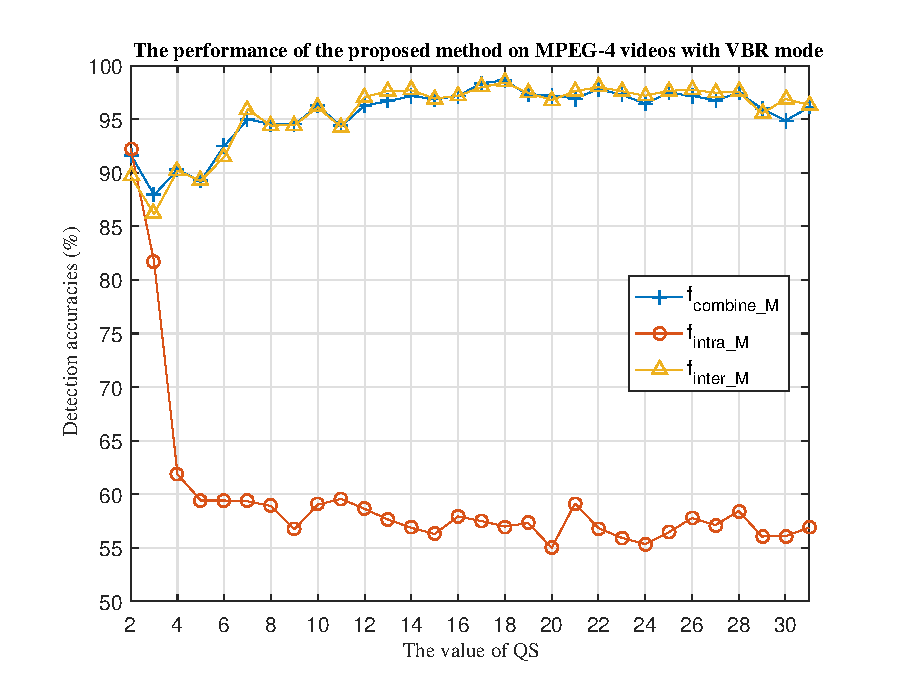
\includegraphics[width=0.5\textwidth]{MPEG4-VBR.eps}
	\caption{Evaluation of the performance on MPEG-4 videos with VBR mode}
	\label{mpeg4-vbr}
\end{figure}



As shown in Fig. \ref{mpeg4-vbr}, detection accuracies for different quality scales have similar variation tendency compared to the results of MPEG-2 videos in VBR mode. It is because the coding process of these two codecs performs alike when bit rate control is turned off. The average detection accuracies of $f_{combine\_\text{M}}$ (95.52\%) and $f_{inter\_\text{M}}$ (95.61\%) are very close. Although $f_{intra\_\text{M}}$ improves the detection capability of the concatenated feature for high-quality videos, it becomes undiscriminating and even noisy in the classification for low-quality videos. On the other hand, $f_{inter\_\text{M}}$ is more robust to expose double compression for middle-quality videos and high-quality videos. 
%After concatenation of $f_{intra\_\text{M}}$ and $f_{inter\_\text{M}}$, there is a negligible degradation of performance in most of cases. It is due to that distinguish capability of $f_{intra\_\text{M}}$ is weaken when the quality of videos is very poor ($QS>8$). 

For CBR videos, the improvement of feature combination is distinct. The average detection accuracy of $f_{combine\_\text{M}}$ is higher than $f_{intra\_\text{M}}$ and $f_{inter\_\text{M}}$ by 14.19\% and 3.7\% respectively. It infers that the features extracted from the intra-coding process and the inter-coding process are complementary to each other, which improves the detection capability of double compression in CBR mode.

\begin{table}[ht!]
	\centering
	\caption{\label{mpeg4-cbr}The detection accuracies of double compression on MPEG-4 videos with CBR mode (\%)}
	\begin{tabular}{ccccc}
		\toprule
		Bit rate (kbps)& $f_{combine\_\text{M}}$ & $f_{intra\_\text{M}}$ & $f_{inter\_\text{M}}$  \\\midrule
		7000 &\textbf{93.48}     &90.73    &86.64    \\
		5000 &\textbf{91.54}     &87.88    &87.63    \\
		3000 &\textbf{89.52}     &85.40    &87.53   \\\midrule
		1000 &\textbf{82.88}      &63.79    &77.83   \\
		900 &\textbf{81.97}     &63.74    &77.30    \\
		800 &\textbf{78.91}     &62.53    &74.14    \\
		700 &\textbf{80.33}     &62.58    &76.94    \\
		600 &\textbf{79.82}     &63.33    &77.63    \\
		500 &\textbf{75.98}     &65.13    &74.65    \\
		400 &\textbf{78.31}     &56.36    &76.74    \\\midrule
		300 &\textbf{81.92}     &58.69    &75.63    \\
		200 &\textbf{71.92}     &56.16    &69.55   \\\midrule
		Average &\textbf{82.22}   &68.03   &78.52  & \\\bottomrule
	\end{tabular}
\end{table}



\subsection{Evaluation of performance on H.264 videos\label{evaluation_h264}}
%Since the popularity of the H.264 videos on the Internet and mobile devices, the robust detection capability of the extended method for H.264 is also of significance. 
In this section, the performance of H264-DM method is evaluated on H.264 videos and compared to the state-of-the-art method \cite{zhang2016detecting}. In \cite{zhang2016detecting}, authors defined a ratio difference set (referred to as RDS) measuring the percentage of quantized DCT coefficients whose value will change after recompression. The classification feature is calculated on RDS and then fed to SVM classifier to detect double compression. Zhang et al. only conducted the evaluation of the method \cite{zhang2016detecting} on VBR videos and only considered $QS\leq 40$. In our experiments, the proposed method and Zhang's method are tested on both VBR and CBR videos. Besides, in VBR mode, all available options of $QS$ are considered, namely $QS = \{1,2,...,52\}$. The dataset-A is used to generate training samples and testing samples.

\begin{figure*}[htbp!]
	\centering
	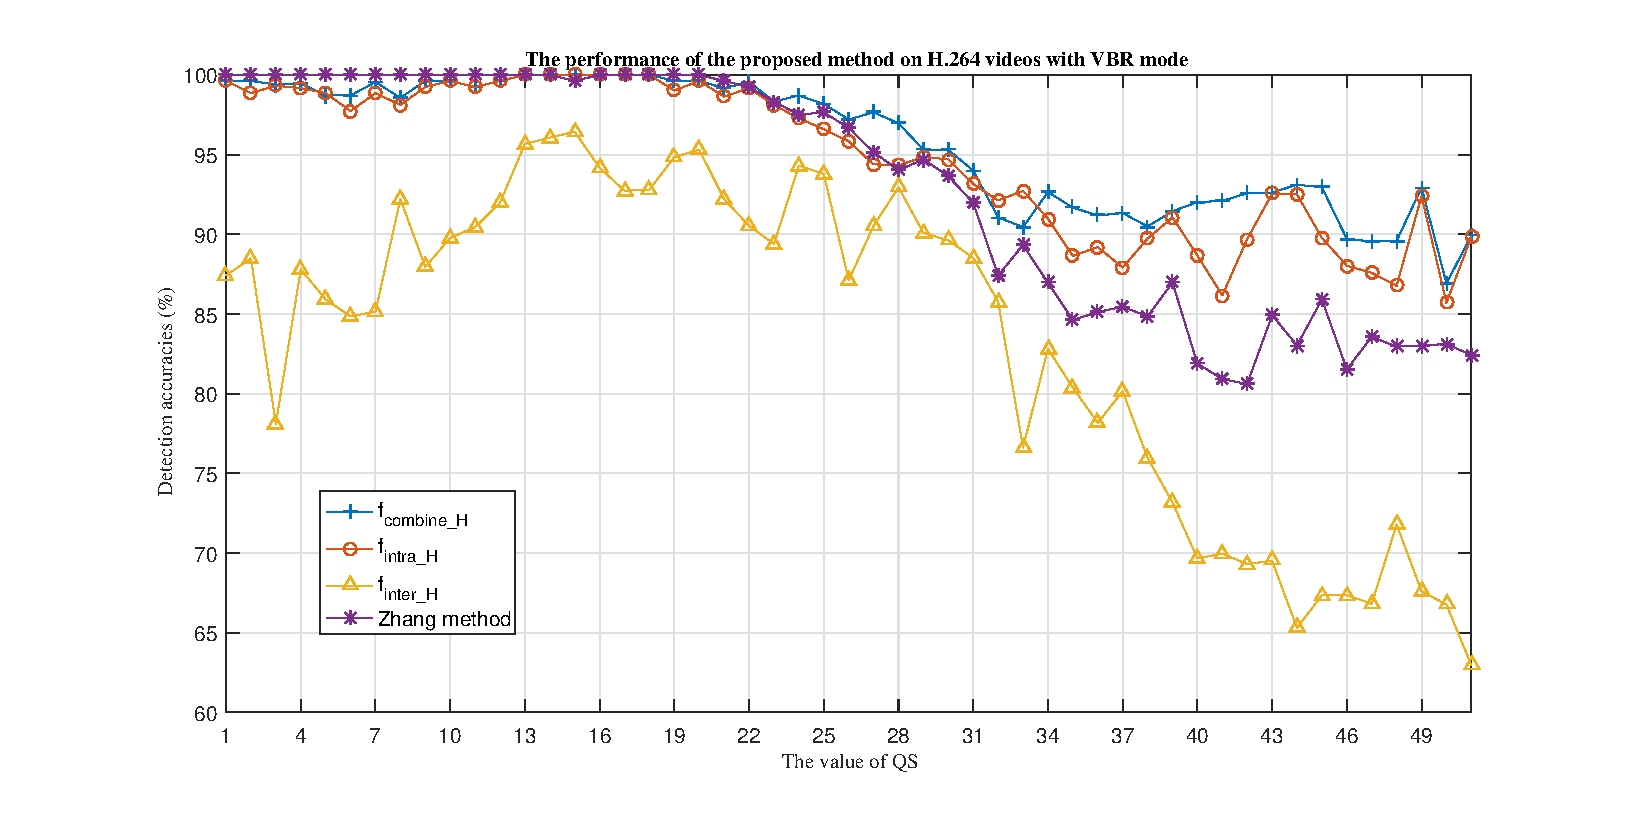
\includegraphics[width=1\textwidth]{H264-VBR.eps}
	\caption{Evaluation of the performance on H.264 videos with VBR mode}
	\label{h264-vbr}
\end{figure*}

\begin{table*}
	\centering
	\caption{\label{tab:rate}The detection accuracies on H.264 videos with CBR mode (\%)}
	\begin{tabular}{cccccc}
		\toprule
		Bit rate (kbps)& $f_{combine\_\text{H}}$ & $f_{intra\_\text{H}}$ & $f_{inter\_\text{H}}$ & Zhang's method\\\midrule
		7000 & \textbf{95.78}     &93.13     & 87.07    &65.18 \\
		5000 & \textbf{97.40}     &91.59     & 95.28    &65.30 \\
		3000 & \textbf{98.89}     &95.61     & 92.47   &77.35 \\\midrule
		1000 & \textbf{97.35}      &97.20     & 91.77   &90.81 \\
		900 & \textbf{97.63}     &96.21     & 91.52    &93.43 \\
		800 & 95.35     &\textbf{95.53}     & 91.26    &92.22 \\
		700 & 97.20     &\textbf{98.21}     & 90.30    &91.92 \\
		600 & 97.80     &\textbf{97.90}     & 91.29    &92.65 \\
		500 & 96.84    &\textbf{97.70}     &  87.25    &93.54 \\
		400 & 95.38     &\textbf{97.05}     & 89.72    &90.25 \\\midrule
		300 & \textbf{94.42}     &91.54    &  91.34   &86.04 \\
		200 & \textbf{95.63}     &88.54     & 92.75   &84.47 \\\midrule
		Average & \textbf{96.61}   & 95.01   &  91.00 & 85.25 \\\bottomrule
	\end{tabular}
\end{table*}

As shown in Fig. \ref{h264-vbr}, the difference between the performance of the proposed method $f_{combine\_\text{H}}$ and Zhang's method is marginal on high-quality videos (e.g., $QS<25$). With the value of $QS$ increasing continuously, the detection accuracy of Zhang's method drops down faster than the proposed method, especially when $QS$ becomes larger than 34. It is because the severe quantization in low-quality videos makes the quantized DCT coefficients much easier to become unchanged and indistinguishable between single compression and double compression. In this case, the discrimination capability of features in \cite{zhang2016detecting} becomes weak. On the other hand, the proposed method $f_{combine\_\text{H}}$ achieves more robust detection results on middle-quality and low-quality videos, since the convergent property of macroblock mode in I-frames $f_{intra\_\text{H}}$ still retains well under more severe quantization. The average detection accuracy of the proposed method (95.80\%) is larger than Zhang's method (92.99\%) by 2.81\% in VBR mode. Besides, the performance of the concatenated feature $f_{combine\_\text{H}}$ is higher than $f_{intra\_\text{H}}$ (94.79\%) and $f_{inter\_\text{H}}$ (82.43\%).
 
For CBR videos, the proposed method achieves significant improvement when the video has very high quality (bit rate $\geq 3000$kbps) while the detection accuracies of Zhang's methods are lower than 80\%. It is because the value of $QS$ for each macroblock may vary after each recompression operation, which is easy to fluctuate the statistics of RDS in \cite{zhang2016detecting}. Besides, rounding and truncation error can impact the statistical properties of quantized coefficients of I-frames in high-quality videos. The proposed method is less sensitive to the variation of $QS$ in this case, which is important in real forensics applications. Additionally, with the video quality becoming worse, the performance of the proposed method is more promising than Zhang's method. In low-quality videos, $f_{inter\_\text{H}}$ improves the robustness of $f_{combine\_\text{H}}$ against severe quantization. The average accuracy of our method on H.264 videos with CBR mode achieves significant improvement compared to Zhang's method.

\subsection{Robustness evaluation for more diverse video contents and more realistic coding parameter settings\label{realistic}}



\begin{table*}[!htb]
	\centering
	\caption{The detection accuracies for more diverse video contents with CBR mode (\%)}
	\begin{tabular}{cccccc}
		\toprule
		& \multicolumn{2}{c}{H264} & MPEG-4 & \multicolumn{2}{c}{MPEG-2} \\
		\cmidrule(r){2-3}\cmidrule(r){4-4}\cmidrule(r){5-6}
		\multicolumn{1}{c}{Bit rate (kbps)} & Proposed & Zhang's method & Proposed & Proposed & Huang's method \\
		\midrule
		3000  & \textbf{95.31} & 81.25 & \textbf{82.03} & \textbf{86.72} & 80.47 \\
		1000  & \textbf{94.53} & 87.50 & \textbf{74.23} & \textbf{85.94} & 77.35 \\
		700   & \textbf{91.40} & 89.84 & \textbf{76.57} & \textbf{76.57} & 71.88 \\
		500   & \textbf{89.07} & 88.29 & \textbf{72.67} & \textbf{75.78} & 65.63 \\
		300   & \textbf{86.72} & 70.32 & \textbf{78.13} & \textbf{79.69} & 61.73 \\
		\bottomrule
	\end{tabular}%
	\label{tab:part2-cbr}%
\end{table*}


In real forensics cases, contents of suspicious videos may be very diverse. In this section, the proposed method is tested on more diverse video contents. Besides, except for the compression quality and rate-control mode, there are several other coding parameters controlling the encoding process, such as GOP size, video spatial resolution and the novel rate-control strategy of H.264 (Constant Rate Factor encoding mode). It is necessary to evaluate the influence of these coding parameter settings to the proposed method. 


\subsubsection{Evaluation of the robustness to more diverse video contents}
In this experiment, 22 extra YUV sequences are collected from the website, referred to as dataset-B. More details about raw videos in the dataset-B are shown in the Appendix. To align the resolution to YUV sequences in the dataset-A, YUV sequences in the dataset-B are first rescaled to CIF resolution (352 $\times$ 288). This process is implemented by the FFmpeg tools. Please note, in this rescaling process, there is no lossy compression artifact introduced to YUV sequences. Besides, frame drop or duplication may exist during this process with the default setting. Then, these rescaled YUV sequences are used to generate samples according to the manner in Section \ref{dataset_video}. For the dataset-B, 64 YUV clips with 100 frames can be obtained. In this experiment, the dataset-A are used to generate training samples (132 positive samples and 132 negative samples) while the dataset-B are used to generate testing samples (64 positive samples and 64 negative samples) for each coding parameter setting. In this way, samples in the training set are totally independent to samples in the testing set. Traditional rate control strategies and different compression qualities are considered in this experiment. The GOP size is fixed to 10. Five-fold cross validation is used to search the optimal parameters of SVM classifier on training samples.



According to the results in Table \ref{tab:part2-cbr}, the proposed method achieves better performance for H.264 videos with CBR mode compared to Zhang's method. It proves that macroblock statistics after continuous recompressions are more reliable to detect double compression with a wider range of video qualities and more diverse video contents. The detection accuracy of the proposed method drops slightly compared to the results in Section \ref{evaluation_h264}. It is because YUV sequences in dataset-B contain more various global motion types, such as fast zooming in and rotated zooming out. It increases the diversity of macroblock statistics in inter-coding frames.
%\textcolor{red}{In other words, the diversity of video contents in the training set can influence the detection performance of the learned classifier.} 
For detection of double compression on MPEG-4 videos, the proposed method has the lowest detection accuracy among three kinds of video compression standards. It is possible that the rate-control strategy of MPEG-4 encoder has the most unstable coding efficiency to different types of video contents. For MPEG-2 videos, the proposed method still outperforms Huang's method for different compression qualities.

\begin{table}[!htb]
	\centering
	\caption{The detection accuracies for more diverse video contents with VBR mode (\%)}
	\begin{tabular}{ccccc}
		\toprule
		& \multicolumn{2}{c}{H264} & MPEG-4 & MPEG-2 \\
		\cmidrule(r){2-3}\cmidrule(r){4-4}\cmidrule(r){5-5}
		\multicolumn{1}{l}{$QS$\tnote{1}} & Proposed & Zhang & Proposed & Proposed \\
		\midrule
		a     & 99.22 & \textbf{100}   & \textbf{90.62} & \textbf{94.53} \\
		b     & \textbf{100} & 98.43 & \textbf{94.53} & \textbf{93.75} \\
		c     & \textbf{94.53} & 92.19 & \textbf{93.75} & \textbf{98.43} \\
		d     & \textbf{74.23} & 72.67 & \textbf{95.31} & \textbf{90.62} \\
		\bottomrule
	\end{tabular}%
	\begin{tablenotes}
		\footnotesize
		\item[1] For H.264 codecs, \{a,b,c,d\} denotes \{2,15,23,48\}.\\ For MPEG-2/4 codecs, \{a,b,c,d\} denotes \{2,8,15,31\}.
	\end{tablenotes}
	\label{tab:part2-vbr}%
\end{table}%

For H.264 videos with VBR mode, the proposed method and Zhang's method both can achieve promising performance on high and medium quality videos. For low-quality videos, the performance becomes worse due to the severe quantization artifact and alternation of pixel value caused by the in-loop deblocking filter during the recompression process. On the other hand, the proposed method keeps high detection accuracy for MPEG-2/4 videos. It should be noted that MBM feature has the dominant discriminating capability of double compression when videos have medium or low-quality, e.g. $QS \geq$ 8. By analyzing the convergent curve of macroblocks with unstable MBM after continuous recompressions, it is found that the number of macroblocks with unstable MBM per P-frame is very small (less than 10 for CIF videos) after only twice compressions for most types of video contents. The statistical properties of MBM with VBR mode are more robust compared to CBR mode, since a constant $QS$ causes less alteration during continuous recompressions. 
%The inter-coding data, such as motion vector, is more likely to become unchanged for MPEG videos after only few times of recompressions.





\subsubsection{Performance evaluation with different GOP sizes \label{evaluation_gop}}

\begin{table*}[!htbp]
	\centering
	\caption{Detection accuracies of the proposed method with\\ different GOP sizes (\%)}
	\begin{tabular}{ccccccc}
		\toprule
		& \multicolumn{2}{c}{H264} & \multicolumn{2}{c}{MPEG-4} & \multicolumn{2}{c}{MPEG-2} \\
		\cmidrule(r){2-3}\cmidrule(r){4-5}\cmidrule(r){6-7}
		Bit rate (kbps)& GOP20 & GOP5  & GOP20 & GOP5  & GOP20 & GOP5 \\
		\midrule
		3000  & 93.02 & 92.56 & 89.02 & 87.70 & 82.39 & 89.21 \\
		1000  & 90.89 & 92.89 & 84.04 & 83.31 & 77.09 & 80.07 \\
		700   & 91.10 & 90.50 & 81.27 & 80.83 & 80.10 & 82.38 \\
		500   & 87.28 & 89.28 & 77.23 & 76.05 & 79.33 & 86.16 \\
		300   & 88.59 & 89.63 & 78.51 & 74.90 & 82.67 & 86.18 \\
		\bottomrule
	\end{tabular}%
	\label{tab:GOP}%
\end{table*}%

Group of pictures (GOP) is the basic encoding unit in video compression. The first frame in each GOP is an intra-coded frame, and the rest of the frames are inter-coded frames, such as P-frame. The interval of GOP has a significant impact on video quality after lossy compression because of the error propagation in the inter-coding process. The influence of different GOP sizes to the proposed method is analyzed in this experiment. Here, GOP sizes are set as 5 and 20. Only CBR mode is considered. The rest of experiment settings are identical to those in Section \ref{evaluation_mpeg2_all} to Section \ref{evaluation_h264}. The results are shown in Table \ref{tab:GOP}.



For H.264 videos, when the GOP size becomes smaller or larger, the detection accuracy drops about 5\% compared to the results in Section \ref{evaluation_h264}. When the length of input video clips is fixed, for larger GOP sizes, the number of I-frames in each video clip decreases. The reliability of $f_{intra\_\text{H}}$ deteriorates due to fewer I-frames available in feature extraction. For smaller GOP sizes, the number of P-frames in each video clip decreases. In this case, the $\text{MBM}_\text{H}$ is easier to become unchanged after single compression because error propagation is slighter with shorter GOP intervals. Thus, the performance of the combination feature ($f_{combine\_\text{H}}$) becomes worse for both larger and smaller GOP sizes with a fixed video length (e.g. 100 frames in our experiments). For MPEG-2 videos, when the GOP size becomes smaller, the proposed method achieves improvement for all cases compared to the results in Section \ref{evaluation_mpeg2_all}. It is because the larger number of I-frames contributes to the better detection capability for high-quality videos while the short duration of GOP leads to MBM more reliable for different video contents for low-quality videos. Different from the H.264 codec, the rate-control strategy in CBR mode of MPEG-2 codecs is much simpler. For MPEG-4 videos, the performance is roughly equal to the results in Section \ref{evaluation_mpeg4} for different GOP sizes.

\subsubsection{Performance evaluation with Constant Rate Factor (CRF) encoding mode}
In H.264 and more advanced codecs, Constant Rate Factor (CRF) is a new kind of rate control strategy. This mode allows the encoder to achieve a specific output quality when the output data size is less important. Each frame is assigned the bitrate to keep the requested quality. It infers the value of quality scales may vary in different frames during the encoding process with CRF mode. In this experiment, the efficiency of the proposed method to detect double compression with CRF mode is evaluated. The CRF of $libx264$ is set as \{2,8,15,23,37,48\}. The rest of experimental settings and the experiment procedures are the same as those in Section \ref{evaluation_h264}. 

\begin{table}[htbp]
	\centering
	\caption{Detection accuracies of the proposed method with Constant Rate Factor (CRF) encoding mode (\%)}
	\begin{tabular}{cccc}
		\toprule
		CRF & $f_{combine\_\text{H}}$ & $f_{intra\_\text{H}}$ & $f_{inter\_\text{H}}$    \\
		\midrule
		2  & 99.49  & 99.39 & 73.13   \\
		8  & 98.21  & 95.64 & 90.91   \\
		15 & 97.34  & 96.83 & 92.32   \\
		23 & 94.26  & 93.06 & 82.02   \\
		37 & 83.23  & 81.60 & 73.19   \\
		48 & 85.95  & 84.26 & 73.23   \\
		\bottomrule
	\end{tabular}%
	\label{tab:crf}%
\end{table}%

According to the results in Table \ref{tab:crf}, the proposed method can achieve very promising detection accuracies for high and medium quality videos, namely CRF $\leq$ 23. Both $f_{intra\_\text{H}}$ and $f_{inter\_\text{H}}$ contribute to the good detection performance complementarily in most cases. It is not surprising that $f_{inter\_\text{H}}$ is inefficient to detect double compression of very high quality videos (e.g. CRF = 2), since the slight quantization degradation and prediction error propagation make MBM$_\text{H}$ more difficult to become unchanged after recompression. For low-quality videos, the detection accuracy drops distinctly due to information loss caused by the severe quantization.


\subsubsection{Performance evaluation with different video spatial resolutions}
The advanced video compression standards are designed to satisfy the storage and transmission of the emerging high definition resolution videos. In this experiment, the robustness of the proposed method for videos with the larger spatial resolution is evaluated. The standard definition resolution (referred to as SD resolution), namely $640\times480$, is considered. Several raw video sequences from the website are collected. More details about selected raw videos are shown in Appendix. All of them are rescaled to SD resolution using the FFmpeg tools. Then, these rescaled YUV sequences are used to generate samples according to the manner in Section \ref{dataset_video}. Finally, a video dataset containing 120 YUV clips with 100 frames in SD resolution can be constructed, referred to as dataset-SD. Please note the rescaling process does not introduce any trace of lossy compression. Only H.264 codec and CBR mode are considered in this experiment. The rest of experimental settings are the same as those in Section \ref{evaluation_h264}.

\begin{table}[htbp]
	\centering
	\caption{Detection accuracies of the proposed method with standard definition resolution videos (\%)}
	\begin{tabular}{cccccc}
		\toprule
		Bit rate (kbps) & 3000  & 1000  & 700   & 500   & 300 \\
		\midrule
		Proposed  & 96.68 & 94.89 & 93.86 & 90.84 & 88.05 \\
		\bottomrule
	\end{tabular}%
	\label{tab:SD}%
\end{table}%

As shown in Table \ref{tab:SD}, for H.264 videos with SD resolution, the proposed method still achieves promising detection performance (detection accuracies are above 90\% in most cases). Since $f_{combine\_\text{H}}$ is based on macroblock statistics after continuous recompressions, a larger number of macroblocks in each frame can provide more reliable convergent prosperities. It infers that the proposed method has promising robustness for detecting double compression with a larger spatial resolution.


\subsection{Performance evaluation with different encoding strategies\label{diff_strategy}}
In our experiments, there are totally three steps involving video encoders, including one for generating training video samples, one for generating testing video samples and one for extracting detection features. From Section \ref{evaluation_mpeg2_all} to Section \ref{realistic}, we set a strong assumption about configurations of encoders, where all three encoders in each experiment are identical to the Encoder\_RDO\footnote{Encoder\_RDO is the H.264 encoder of the library ``libx264'' configured with the default rate-distortion optimization algorithm. It is implemented by setting the option ``-subq'' of libx264 as default, namely ``6''.}. To evaluate the robustness of the proposed method against different encoding strategies, we designed the following experiment. YUV sequences in the dataset-A are applied. The experimental settings and procedures are the same as those in Section \ref{evaluation_h264}, except that testing video samples are generated with the Encoder\_FAST\footnote{Encoder\_FAST is the H.264 encoder of the library ``libx264'' configured with the SAD mode decision strategy. It is implemented by setting the option ``-subq'' of libx264 as ``1''.} instead of the original Encoder\_RDO. According to the experimental results, the proposed method and Zhang's method are both invalid to provide reliable detection results (detection accuracies are about 50\%, nearly random guessing). This result is not surprising, because video samples compressed with various encoders perform quite different variation tendencies after continuous recompressions. The classifier with the supervised-learning manner is hard to work well to unknown patterns.

\begin{table}[htbp]
	\centering
	\caption{Evaluation of the robustness to different encoding strategies (\%)}
	\begin{tabular}{cccccc}
		\toprule
		Bit rate (kbps) & 3000  & 1000  & 700   & 500   & 300 \\
		\midrule
		Proposed & 83.82 & 86.56 & 86.78 & 86.94 & 82.92 \\
		Zhang's method & 67.50  & 78.66 & 78.91 & 79.56 & 76.29 \\
		\bottomrule
	\end{tabular}%
	\label{tab:rdo_sad}%
\end{table}%

The possible solution to this drawback is to consider different encoding strategies in the training process. If macroblock statistics after continuous recompressions with different kinds of encoding strategies are considered, the trained classifier may become more powerful to detect double compression. To verify this assumption, the following experiment is conducted. In this experiment, training video samples encoded using Encoder\_FAST and Encoder\_RDO are mixed up to train the classifier. Testing video samples encoded by these two kinds of encoding strategies are also merged together. Only CBR mode is considered in this experiment. The rest of experimental settings and procedures are the same as those in Section \ref{evaluation_h264}.

As shown in Table \ref{tab:rdo_sad}, the proposed method achieved better performance than Zhang's method. However, the detection accuracies of the proposed method dropped distinctly (about 10\%) compared to the results in Section \ref{evaluation_h264}. It infers that a different encoder applied to conduct recompressions is harmful to the convergent tendency of unstable macroblocks shown in Section \ref{degrad_h264}. Besides, the feature extraction process of the proposed method and Zhang's method both involve the recompression operation. It leads to the deterioration of detection performance.


\section{conclusion}
In this work, we proposed two robust detection methods for double compression with the same coding parameters in MPEG videos and H.264 videos respectively. They have the similar detection framework, where classification features are extracted from both intra-coding information and inter-coding information based on degradation mechanisms after recompression. It is significant to construct detection features fusing the coding information from both spatial domain and temporal domain, since macroblock statistics varies distinctively for different compression qualities. Extensive experiments are conducted on double compression databases consisting of diverse video contents.  Experimental results illustrate the proposed features are robust and efficient under various encoding conditions. Besides, the proposed method outperforms existing approaches in different rate control modes, especially for CBR videos. This superiority is necessary for the real forensics scenarios. 

The future works focus on the following issues: 1) In our algorithm, the encoder generating testing video samples need to be considered in the training phase. Otherwise, the trained classifier is invalid to identify unseen patterns of macroblock statistics in suspicious videos, caused by unknown rate-distortion optimization strategies. This limitation also exists in other existing methods which involve the recompression operation in the feature extraction process. We will focus on more generalized models of double compression considering advanced video quality assessment techniques to overcome this limitation. 2) It is noted that in view of the limited number of YUV sequences, we performed data augmentation by dividing each raw video into non-overlapping clips. However, such procedure may introduce data dependency of samples obtained from the same source sequence. Considering the limited amount of YUV sequences in the current online video database, we plan to construct a new database in the future. The new dataset is expected to contain more videos with various contents. 3) The similar idea of our work can be extended to detect double compression in HEVC videos.




\appendix

\section{}
All YUV sequences in this paper were obtained from the online video database: http://media.xiph.org/video/derf/.

The name list of YUV sequences for dataset-A is shown as follows: \emph{akiyo, bowing, bridge-close, bridge-far, bus, city, coastguard, container, deadline, flower, football, foreman, galleon, hall, harbour, highway, husky, ice, intros, mobile, mother-daughter, news, vtc1nw, pamphlet, paris, sign-irene, silent, soccer, students, tempete, washdc, waterfall}. 

The name list of YUV sequences for dataset-B is shown as follows: \emph{720p: ducks\_take\_off, FourPeople, in\_to\_tree, Johnny, KristenAndSara, old\_town\_cross, park\_joy, parkrun, shields, stockholm, sunflower, vidyo1, vidyo3, vidyo4; 1080p: blue\_sky,crowd\_run, pedestrian\_area, rush\_hour, snow\_mnt, station2, touchdown\_pass, tractor, west\_wind\_easy.}

YUV sequences used to construct dataset-SD include all the YUV sequences in dataset-B and \emph{1080p: rush\_field\_cuts}.

\bibliography{double_same_quality}

\begin{IEEEbiography}[{
\includegraphics[width=1in,height=1.25in,clip,keepaspectratio]{bios-xinghaojiang.png}}]{Xinghao Jiang}
	received the Ph.D. degree in electronic science and technology from Zhejiang University, Hangzhou, China, in 2003.
	
	He is currently a Professor with the School of Electronic Information and Electrical Engineering, Shanghai Jiao Tong University, Shanghai, China. He was a visiting scholar with the New Jersey Institute of Technology, Newark, NJ, USA, from 2011 to 2012.  His research interests include multimedia security and image retrieval, intelligent information processing, cyber information security, information hiding and watermarking. Dr. Jiang is an IEEE member.
\end{IEEEbiography}

\begin{IEEEbiography}[{
\includegraphics[width=1in,height=1.25in,clip,keepaspectratio]{bios-peisonghe.png}}]{Peisong He}
	received the B.S. degree from the University of Electronic Science and Technology of China, Chengdu, China, in 2013.
	
	He is currently pursuing the Ph.D. degree with the School of Electronic Information and Electrical Engineering, Shanghai Jiao Tong University, Shanghai, China. From Sept. 2016 to Aug. 2017, he worked as a visiting student at the Rapid-Rich Object Search Lab of the Nanyang Technological University, Singapore. His research interest includes multimedia forensics and security.
\end{IEEEbiography}


\begin{IEEEbiography}[{
\includegraphics[width=1in,height=1.25in,clip,keepaspectratio]{bios-tanfengsun.png}}]{Tanfeng Sun}
	received the Ph.D. degree in information and communication system from Jilin University, Changchun, China, in 2003.
	
	He is currently an Associate Professor with the School of Electronic Information and Electrical Engineering, Shanghai Jiao Tong University, Shanghai, China. He had cooperated with Prof. Y.Q. Shi in New Jersey Institute of Technology, U.S.A, as a visiting scholar from Jul. 2012 to Dec. 2013. His research includes digital forensics on video forgery, digital image and video watermarking, and so on.  He had published over 90 papers with his colleagues till now. Dr. T.F. Sun is an IEEE Senior Member.	
	
\end{IEEEbiography}

\begin{IEEEbiography}[{
\includegraphics[width=1in,height=1.25in,clip,keepaspectratio]{bios-fengxie.png}}]{Feng Xie}
	received the B.S. degree and M.S. degree with the School of Electronic Information and Electrical Engineering from Shanghai Jiao Tong University, Shanghai, China, in 2014 and 2017, respectively. His research interest includes video forensics.
	
	
\end{IEEEbiography}

\begin{IEEEbiography}[{
\includegraphics[width=1in,height=1.25in,clip,keepaspectratio]{bios-shilinwang.png}}]{Shilin Wang}
	received his B.Eng. degree in Electrical and Electronic Engineering from Shanghai Jiaotong University, Shanghai, China in 2001, and his Ph.D. degree in the Department of Computer Engineering and Information Technology, City University of Hong Kong in 2004.
	
	He is currently an Associate Professor with the School of Electronic Information and Electrical Engineering, Shanghai Jiaotong University, Shanghai, China. His research interests include image processing and pattern recognition. 
\end{IEEEbiography}



\end{document}
